\chapter{\textsc{Renew} Prototyp} 
	In diesem Kapitel entsteht ein Prototyp, der \textsc{Renew} schrittweise modularisiert, bis die Applikation den größten Teil ihre Funktionalität auf dem Modulpfad betreiben kann. \newline
	Für die Umsetzung des Prototypen werden zuerst Anforderungen erfasst, die der modularisierte \textsc{Renew} Prototyp erfüllen muss, um unserer Vision der Implementation zu entsprechen. Infolgedessen entsteht ein Implementierungsplan sowie ein Prototyp. 

\section{Anforderungen} \label{sec:anforderungen}
	Im Kern der Modernisierung von \textsc{Renew} liegt die Anpassung von \textsc{Renew} an das Modulsystem von Java und dessen Anforderungen an Applikationskomponenten. Aus den \textsc{Renew} Plugins sollen explizite Module entstehen, die auf dem Modulpfad betriebsfähig sein müssen. Die Drittanbieter-Bibliotheken sollen mit in den Modulpfad aufgenommen werden und als automatische Module ihre Aufgabe erfüllen. Zusätzlich darf die Migration und damit verbundene Anpassung und Aufbereitung der Mängel die Kommunikation sowie interne Funktionsweise von \textsc{Renew} nicht verändern. Dementsprechend soll garantiert werden, dass die darunter liegende theoretische Grundlage in Takt bleibt. 

% Was soll der Prototyp leisten 
\subsection{Interaktion}
	Der erste modulare \textsc{Renew} Prototyp soll mit einer minimalen Plugin Anzahl auf dem Modulpfad betriebsfähig sein und eine Möglichkeit bieten, Petrinetze zu erstellen, zu simulieren und zu serialisieren. Das heißt, es muss eine UI zu sehen sein, die mit den nötigen Werkzeugen und der darunter liegender Logik ausgestattet ist. 

\subsection{Projektstruktur}
	Für die Umsetzung des modularen \textsc{Renews} wird für jedes Plugin eine moderne Projektstruktur benötigt, die den Inhalt entsprechend dem etablierten Maven Standardverzeichnislayout auf Java Module und die dafür benötigten Ressourcen aufteilt. 

\subsection{Entwicklungsumgebung} 
	In der existierenden \textsc{Renew} Entwicklungsumgebung werden alle Plugin Projekte durch eine versteckte \textit{.project} beschrieben. Das heißt, der Klassenpfad und die Bindung der Codebausteine geschehen versteckt und für den Entwickler schwer zugänglich. Damit ist der Entwickler gezwungen, den weiten und verschachtelten Weg durch die UI Konfiguration von Eclipse zu betreten, der sich mit der Zeit wandeln kann. Dieser Sachverhalt wurde von mir im letzten Projekt beobachtet und kostete Zeit für alle Projektteilnehmer, da die Universitätsrechner strikten Rechten unterliegen, die keine Benutzer definierte Eclipse Entwicklungsumgebung aufsetzen lässt. Darüber hinaus ist die Konfiguration von \textsc{Renew} in anderen Entwicklungsumgebungen wie IDEA oder Netbeans mit der \textit{.project} Konfigurationsdatei nicht möglich. \bigbreak

	Um eine Entwicklungsumgebung unabhängige Konfiguration anzulegen, wird ein neues Werkzeug benötigt. 

\subsection{Packaging}
	Da \textsc{Renew} an das Modulsystem angepasst werden muss, muss die Prozedur für das Kompilieren und das Verpacken der Codebasis die Veränderung miterleben.\newline
	\textsc{Renew} benutzt zurzeit das \textit{Apache Ant} Werkzeug, das alle Plugins kompiliert und in eine ausführbare Form bringt. Dieses ist in Jahre gekommen und enthält wesentlich geringeren Funktionsumfang gegenüber der aktuellen Konkurrenz, wie Maven und Gradle. Sie bieten eine Abhängigkeitsverwaltung, konfigurierbare Plugins und Programmiersprachen. Im Gesetz zu der aufgeblasenen XML-Konfiguration von Ant, die jeden kleinen Schritt ausführlich dokumentiert, beherrschen die modernen \textit{build} Werkzeuge die Komplexität durch den \textit{Convention over Configuration} Ansatz und flexiblen Ausdrucksweisen. \bigbreak

	Die minimale Version von \textsc{Renew} soll sich an einem modernen \textit{build} Werkzeug bedienen und ein ausführbares Ergebnis erzielen.

\section{Spezifikation}
	Um die Anforderungen umzusetzen, wird die erarbeitete minimale Version isoliert, umstrukturiert und mit dem Gradle \textit{build} Werkzeug für das Arbeiten in der Entwicklungsumgebung IDEA aufgerüstet. Da Gradle die Verwaltung des Projekts sowie das Kompilieren und Erstellen von ausführbaren Paketen übernehmen kann, ist es eine gute Wahl für das Aufsetzen einer modernen modularen Projektstruktur.\newline 
	Dafür muss das bestehende Ant \textit{build} System analysiert und mit dem Gradle Werkzeug wiederaufgebaut werden. Dieses soll so gut wie möglich die bestehende Drittanbieter-Bibliotheken verwalten, Module kompilieren und die benötigten Erweiterungen, wie das JavaCC Werkzeug, unterstützen.\bigbreak

	Nachdem die Projektstrukturen die passende Form angenommen haben, müssen die Projekt Abhängigkeiten analysiert und innerhalb der \textit{module-info.java} aufgenommen werden.\bigbreak

	Zu Letzt entsteht eine bekannte Ordnerstruktur mit Drittanbieter-Bibliotheken, Plugins und Konfigurationsdateien, die mithilfe des \textit{Plugin Managers} verwaltet werden.

\section{Entwurf}
	Der Entwurf berücksichtigt die schrittweise Migration und lässt die \textsc{Renew} Applikation während der Gesamtmigration betriebsfähig bleiben. Das heißt, Plugins auf den Klassenpfad sowie Modulpfad können nahtlos mit einander kommunizieren und ihre Funktion während der Migration weiterhin erfüllen.\bigbreak

	\begin{figure}[h!]
		\centering
		\begin{minipage}{7cm}
			\dirtree{%
			 .1 Project.
			 .2 src.
			 .3 main.
			 .4 java.
			 .5 de.application.purpose.
			 .6 de.
			 .7 application.
			 .8 purpose.
			 .4 resources.
			 }
		\end{minipage}
		\caption{Projektstruktur}
		\label{fig:projektstruktur}
	\end{figure}
	Für den ersten Prototypen wird zuerst eine Projektstruktur erstellt, die für jedes Plugin Projekt die Möglichkeit bieten soll, aus mehreren Modulen zu bestehen. Dafür wird eine Struktur \ref{fig:projektstruktur} erstellt, die im Java Verzeichnis alle Module bündelt, die über den Modulnamen disjunkt voneinander verwaltet werden. Nichtsdestotrotz gehören sie zum gleichen Projekt und teilen unter sich das Ressourcen Verzeichnis, das im weiteren Verlauf zum Erstellen der ausführbaren Pakete benötigt wird.\bigbreak
	       
	Nachdem die Projektstruktur der gewünschten Form entspricht, muss diese in den Gradle Konfigurationsdateien verankert werden. Hierfür wird für jedes Projekt die Projektstruktur und dessen Abhängigkeiten in der \textit{build.gradle} Konfigurationsdateien \ref{fig:gradle_project} festgehalten, indem Java sowie Ressourcen Stammverzeichnisse und Projekte definiert und Drittanbieter-Bibliotheken Abhängigkeiten für den Kompilation-Pfad bestimmt werden. \bigbreak

 		\begin{figure}[h!]
		\centering
		\begin{minipage}{7cm}
			\dirtree{%
			 .1 Project.
			 .2 build.gradle.
			 .2 settings.gradle.
			 .2 src.
			 .3 main.
			 .4 java.
			 .5 de.application.purpose.
			 .6 de.
			 .7 application.
			 .8 purpose.
			 .4 resources.
			 }
		\end{minipage}
		\caption{Gradle Konfiguration}
		\label{fig:gradle_project}
	\end{figure}
 	Die oben genannten Schritte müssen für jedes Projekt der minimalen Version von \textsc{Renew} durchgeführt und im Anschluss über die entsprechende Entwicklungsumgebung  validiert werden. Wenn diese alle Klassen und die benötigten Abhängigkeiten finden und kompilieren kann, wurden alle Projekte richtig strukturiert, definiert und miteinander sauber verbunden. In diesem Zustand ist die komplette Struktur des Projekts innerhalb von Gradle verpackt und kann von jeder Entwicklungsumgebung ausgelesen werden. \newline

	Da jetzt eine lauffähige minimale \textsc{Renew} Version für den Klassenpfad erstellt werden kann, ist es Zeit diese zu Modularisieren und die einzelnen Plugins auf den Modulpfad zu migrieren. Dafür werde ich den \textit{bottom up} Ansatz aus dem Kapitel Migration \ref{sec:bottomUP} verwenden und Schritt für Schritt die Plugins auf den Modulpfad bewegen.

	\begin{figure}[h!]
		\centering
		\begin{minipage}{7cm}
			\dirtree{%
			 .1 Project.
			 .2 build.gradle.
			 .2 settings.gradle.
			 .2 src.
			 .3 main.
			 .4 java.
			 .5 de.application.purpose.
			 .6 de.
			 .7 application.
			 .8 purpose.
			 .6 module-info.java.
			 .4 resources.
			 }
		\end{minipage}
		\caption{Modulumwandlung}
		\label{fig:module_project}
	\end{figure}

	Zuerst werden die Drittanbieter-Bibliotheken, wie \textit{log4j}, auf den Modulpfad als automatische Module eingebunden und werden damit aus den Klassen- sowie Modulpfaden für die Nutzung zugleich erreichbar sein. Anschließend werden Plugins als explizite Module migriert, die keine Plugin Abhängigkeiten besitzen und aus dem Modulpfad keine Zugriffe auf den Klassenpfad ausführen müssen.   Beispielsweise besitzt das \textit{Util} Plugin keine Abhängigkeiten auf \textsc{Renew} Plugins und wird für die Ausführung auf dem Modulpfad, durch eine \textit{moduel-info.java} Konfigurationsdatei erweitert. Wie in der Abbildung \ref{fig:module_project} dargestellt, muss sich diese im Stammverzeichnis des Moduls befinden und die benötigten automatischen Module deklarieren,.\newline
	In den nächsten Schritten werden Plugins Schritt für Schritt auf den Modulpfad migriert, indem für jedes Plugin eine eigene \textit{module-info.java} Konfigurationsdateien angelegt wird, in der sich ihre Abhängigkeiten auf automatische Drittanbieter-Module sowie explizite Plugin-Module befinden.\bigbreak 

	Dieses Vorgehen wird solange durchgeführt bis jedes Plugin sich auf dem Modulpfad befindet. 

\section{Umsetzung}

	Die Umsetzung realisiert den Entwurf und erstellt eine neue Projektstruktur für alle Plugins der minimalen \textsc{Renew} Version \ref{fig:plugin_deps}. Diese werden anschließend mit dem Gradle Werkzeug zusammengeführt und bilden ein kompilierfähiges Konstrukt. Nachfolgend werden die auserwählten Plugins, mit der \textit{module-info.java} versehen und deklarieren innerhalb der Konfigurationsdateien die zuvor vorgestellten Kommunikationskanäle \ref{sec:mod_kop} zwischen den Plugins.\newline
	Der Modularisierungsprozess geschieht iterativ und wird für jedes Plugin einzeln nacheinander durchgeführt.
\newpage
\subsection{Umstrukturierung}

	Für die Umsetzung der Anforderungen und des Entwurfs wird zuerst die Projektstruktur jedes Plugins angepasst. Dafür wird die Struktur jedes Plugins analysiert, umstrukturiert und im weiteren Verlauf von Mängeln befreit. In den meisten Fällen werden \textit{split pakages} und gemischte Strukturen innerhalb der Codebasis erwartet.\bigbreak
	Zuerst wird eine grobe Maven Projektstruktur erstellt, in dem sich zusätzlich ein Plugin Wurzelverzeichnis befindet. Anschließend migriert man die Codebasis in das Plugin Wurzelverzeichnis, welches den neuen Plugin Namen trägt.

	\begin{figure}[h!]
		\centering
		\small
		\setlength{\DTbaselineskip}{7pt}
		\begin{minipage}{7cm}
			\dirtree{%
			 .1 Gui.
			 .2 build.xml.
			 .2 etc.
			 .3 README.gui.
			 .3 plugin.cfg.
			 .2 src.
			 .3 de.
			 .4 renew.
			 .5 ant.
			 .5 gui.
			 .6 images.
			 .6 menu.
			 .6 pnml.
			 .7 converter.
			 .7 creator.
			 .7 parser.
			 .4 io.
			 .5 exportFormats.
			 .5 importFormats. 
			 }
		\end{minipage}
		\caption{Gui Projekt}
		\label{fig:gui}
	\end{figure}

	Das Gui Plugin enthält die geläufige mangelnde Organisation der Ressourcen. Zum Teil befinden sich diese in den \textit{etc} Verzeichnis und zum Teil sind diese in dem Java \textit{source set} Verzeichnis integriert, wie in der Abbildung \ref{fig:gui} dargestellt.\newline
	Um diese zu beheben, wird das Verzeichnis \textit{de.renew.gui.images}, das mit den \textit{png} und \textit{gif} Daten befüllt ist, in das Ressourcen Verzeichnis migriert. Damit die Applikation diese wiederfindet, werden die Zugriffspfade für die Ressourcen innerhalb des Gui Plugin an das neue Verzeichnis angepasst, indem die internen statischen Konstanten, wie \textit{CPNIMAGES}, auf den entsprechenden Ort verweisen. \newline
	Zum Schluss werden die \textit{README} und die \textit{plugin.cfg}  aus dem \textit{etc} Verzeichnis in das Ressourcen Verzeichnis bewegt. Somit ist eine Struktur erstellt worden, die sich auf das Modulsystem von Java anwenden lässt. \bigbreak

	\begin{figure}[h!]
		\centering
		\small
		\setlength{\DTbaselineskip}{7pt}
		\begin{minipage}{7cm}
			\dirtree{%
			 .1 Formalism.
			 .2 build.xml.
			 .2 etc.
			 .3 README.formalism.
			 .3 plugin.cfg.
			 .2 src.
			 .3 de.
			 .4 renew.
			 .5 formalism.
			 .6 base.
			 .6 bool.
			 .6 function.
			 .7 java.
			 .8 JavaNetParser.jj.
			 .7 pt.
			 }
		\end{minipage}
	  \caption{Formalism Projekt}
	  \label{fig:formalism}
	\end{figure}

	Andere Plugins wie Formalism, CH oder Misc besitzen \textit{JavaCC} Dateien, wie im Beispiel \ref{fig:formalism} dargestellt, enden diese auf \textit{jj}. Sie erstellen Java Netz Grammatiken und wandeln die Java-Basis für die Ausführung ab. Diese liegen lose zwischen den Java Klassen und werden von den Java Compiler nicht interpretiert. Daher macht es Sinn, diese in ein eigenes \textit{Source Set} auszulagern und für den JavaCC Compiler für die Übersetzung zu gruppieren.

	\begin{figure}[h!]
		\centering
		\footnotesize
		\setlength{\DTbaselineskip}{10pt}
		\begin{minipage}{.45\textwidth}
			\dirtree{%
			 .1 Formalism.
			 .2 src.
			 .3 main.
			 .4 java.
			 .5 de.renew.formalism.
			 .6 de.
			 .7 renew.
			 .8 formalism.
			 .9 base.
			 .9 bool.
			 .9 function.
			 .9 java.
			 .9 pt.
			 .4 javacc.
			 .5 JavaNetParser.jj.
			 .4 resources.
			 .5 README.formalism.
			 .5 plugin.cfg.
			 }
		\end{minipage}
		\begin{minipage}{.5\textwidth}
			\dirtree{%
			 .1 Gui.
			 .2 src.
			 .3 main.
			 .4 java.
			 .5 de.renew.gui.
			 .6 de.
			 .7 renew.
			 .8 gui.
			 .9 menu.
			 .9 pnml.
			 .10 conv.rng.
			 .10 converter.
			 .10 creator.
			 .10 parser.
			 .10 ptNetb.pntd.
			 .10 refNetb.pntd.
			 .9 io.
			 .10 exportFormats.
			 .10 importFormats.
			 .9 tasks.
			 .5 resources.
			 .6 README.gui.
			 .5 images.
			 .5 plugin.cfg.
			 }
		\end{minipage}
	  \caption{Resultierende Projektstrukturen}
	  \label{fig:resultStr}
	\end{figure}

	Das finale Resultat in der Abbildung \ref{fig:resultStr} erlaubt, eine einfache Paketstruktur Analyse durchzuführen, um die \textit{Split Packages} zu identifizieren. \bigbreak

	Auf den ersten Blick kann eine Überschneidung zwischen den Gui und den RenewAnt Plugin erkannt werden, da beide den \textit{de.renew.ant} Namensraum besetzen, der sich um bestimmte Ant spezifische Aufgaben kümmert. Aufgrund dessen wird der Namensraum in dem Gui Plugin in \textit{task} zu den Gunsten des RenewAnt Plugins umbenannt. Des Weiteren könnten beide \textit{Task's} in den RenewAnt Plugin verschoben werden, da dieser keine Abhängigkeiten in dem Gui Plugin besitzt und nicht in den Aufgabenbereich der UI fällt. 

\subsection{Gradle}

 	Um die Zyklen zu erkennen, wird ein Gradle \textit{build} Skript erstellt, der die Java \textit{Source Sets} für den Kompilationsschritt definiert und die benötigten Projekte sowie Drittanbieter-Bibliotheken auf den Projektklassenpfad einbindet. Mit der Unterstützung der Gradle Projektumgebung und einer IDE können anschließend alle Abhängigkeiten aufgedeckt und auf Zyklen überprüft werden. \newline
 	Für die Umsetzung der Gradle Projektumgebung wird zuerst das bestehende Ant System analysiert. Dieses besteht aus Skripten, die sich in jedem Plugin befinden und die entsprechenden Projekte ausführbare Jar's erstellen. Die Ant Skripte sind sehr ähnlich aufgebaut und wiederholen ein Erstellungsmusster für alle Plugins. \newline
	\begin{figure}[h!]
	  \centering
	  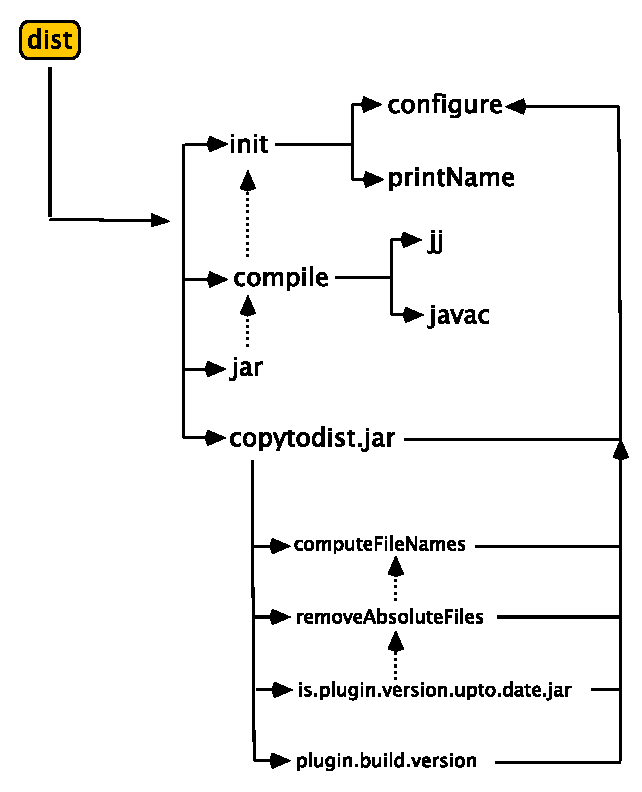
\includegraphics[width=0.5\textwidth]{material/images/ant-build.pdf}
	  \caption{Ant Skript}
	  \label{fig:antscript}
	\end{figure}

	In der Abbildung \ref{fig:antscript} ist ein Modell für die Erstellung eines Plugins mit dem Ant Werkzeug dargestellt. Ant initiiert das Skript mit Feldern und benötigten Variablen aus einer globalen Konfiguration, generiert Java Daten mit dem \textit{jj Target}, kompiliert und verpackt die ausführbaren Klassen. \bigbreak
	
	Für die Gradle Umsetzung werden Schritte, die über die etablierten Operationen zum Erstellen einer Ausführbaren Java Applikation wahrgenommen und in der folgenden Gradle Umgebung eingebunden.\newline
	Dafür wird zuerst ein übergeordneter Gradle Projekt deklariert, das Subprojekte aus allen Plugin Verzeichnissen erstellt.\bigbreak

	\begin{figure}[h!]
	  \centering
	  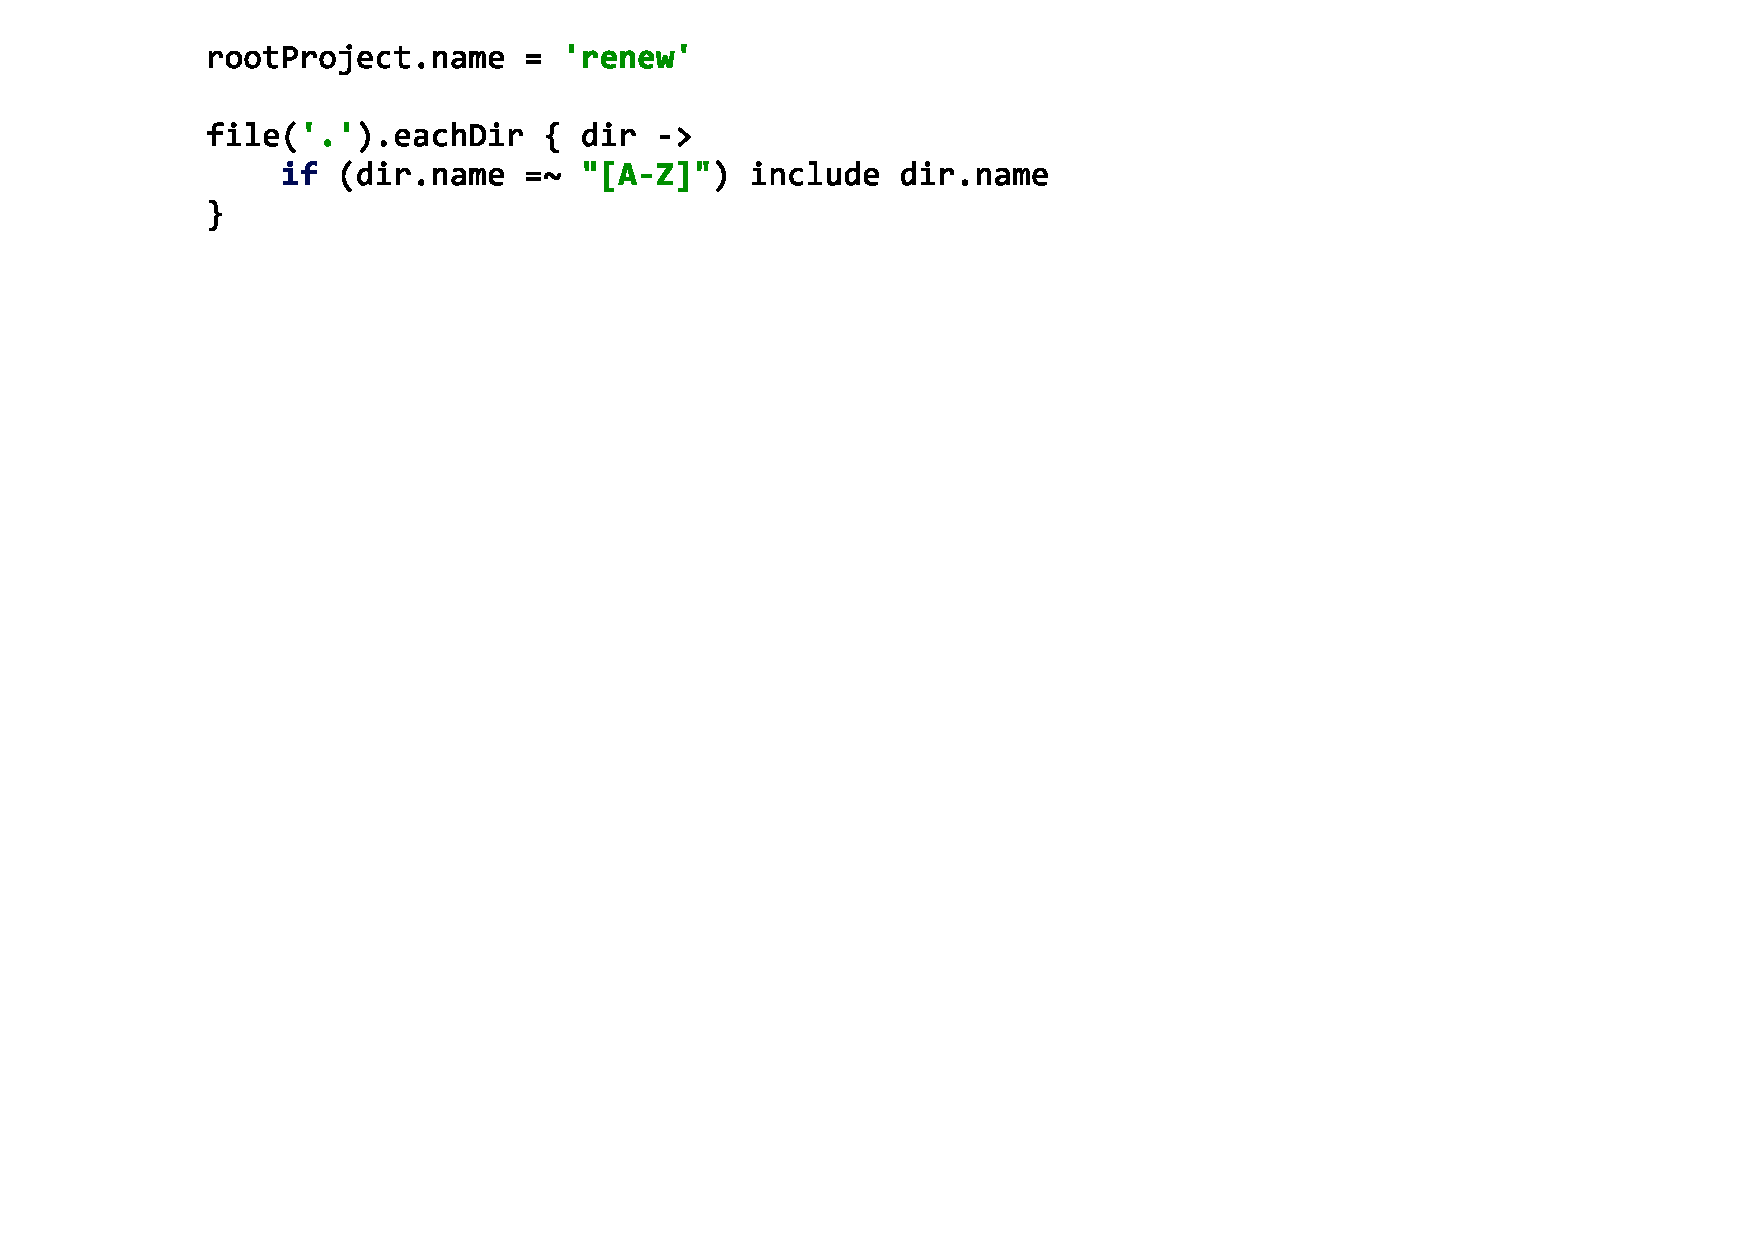
\includegraphics[width=0.6\textwidth]{material/images/settingsgradle.pdf}
	  \caption{Subprojekte}
	  \label{fig:subprojekte}
	\end{figure}

 	Die \textit{settings.gradle} Datei in der Abbildung \ref{fig:subprojekte}, die in der Konfigurationsphase des Gradle Lebenszyklus ausgelesen wird, ist für diesen Konfigurationsschritt zuständig und kann mithilfe von \textit{Groovy} beliebigen Code für die Deklaration der Projekte enthalten. In diesem Fall werden alle Verzeichnisse, die mit einem Großbuchstaben anfangen als Gradle-Subprojekte eingebunden.\bigbreak

	\begin{figure}[h!]
	  \centering
	  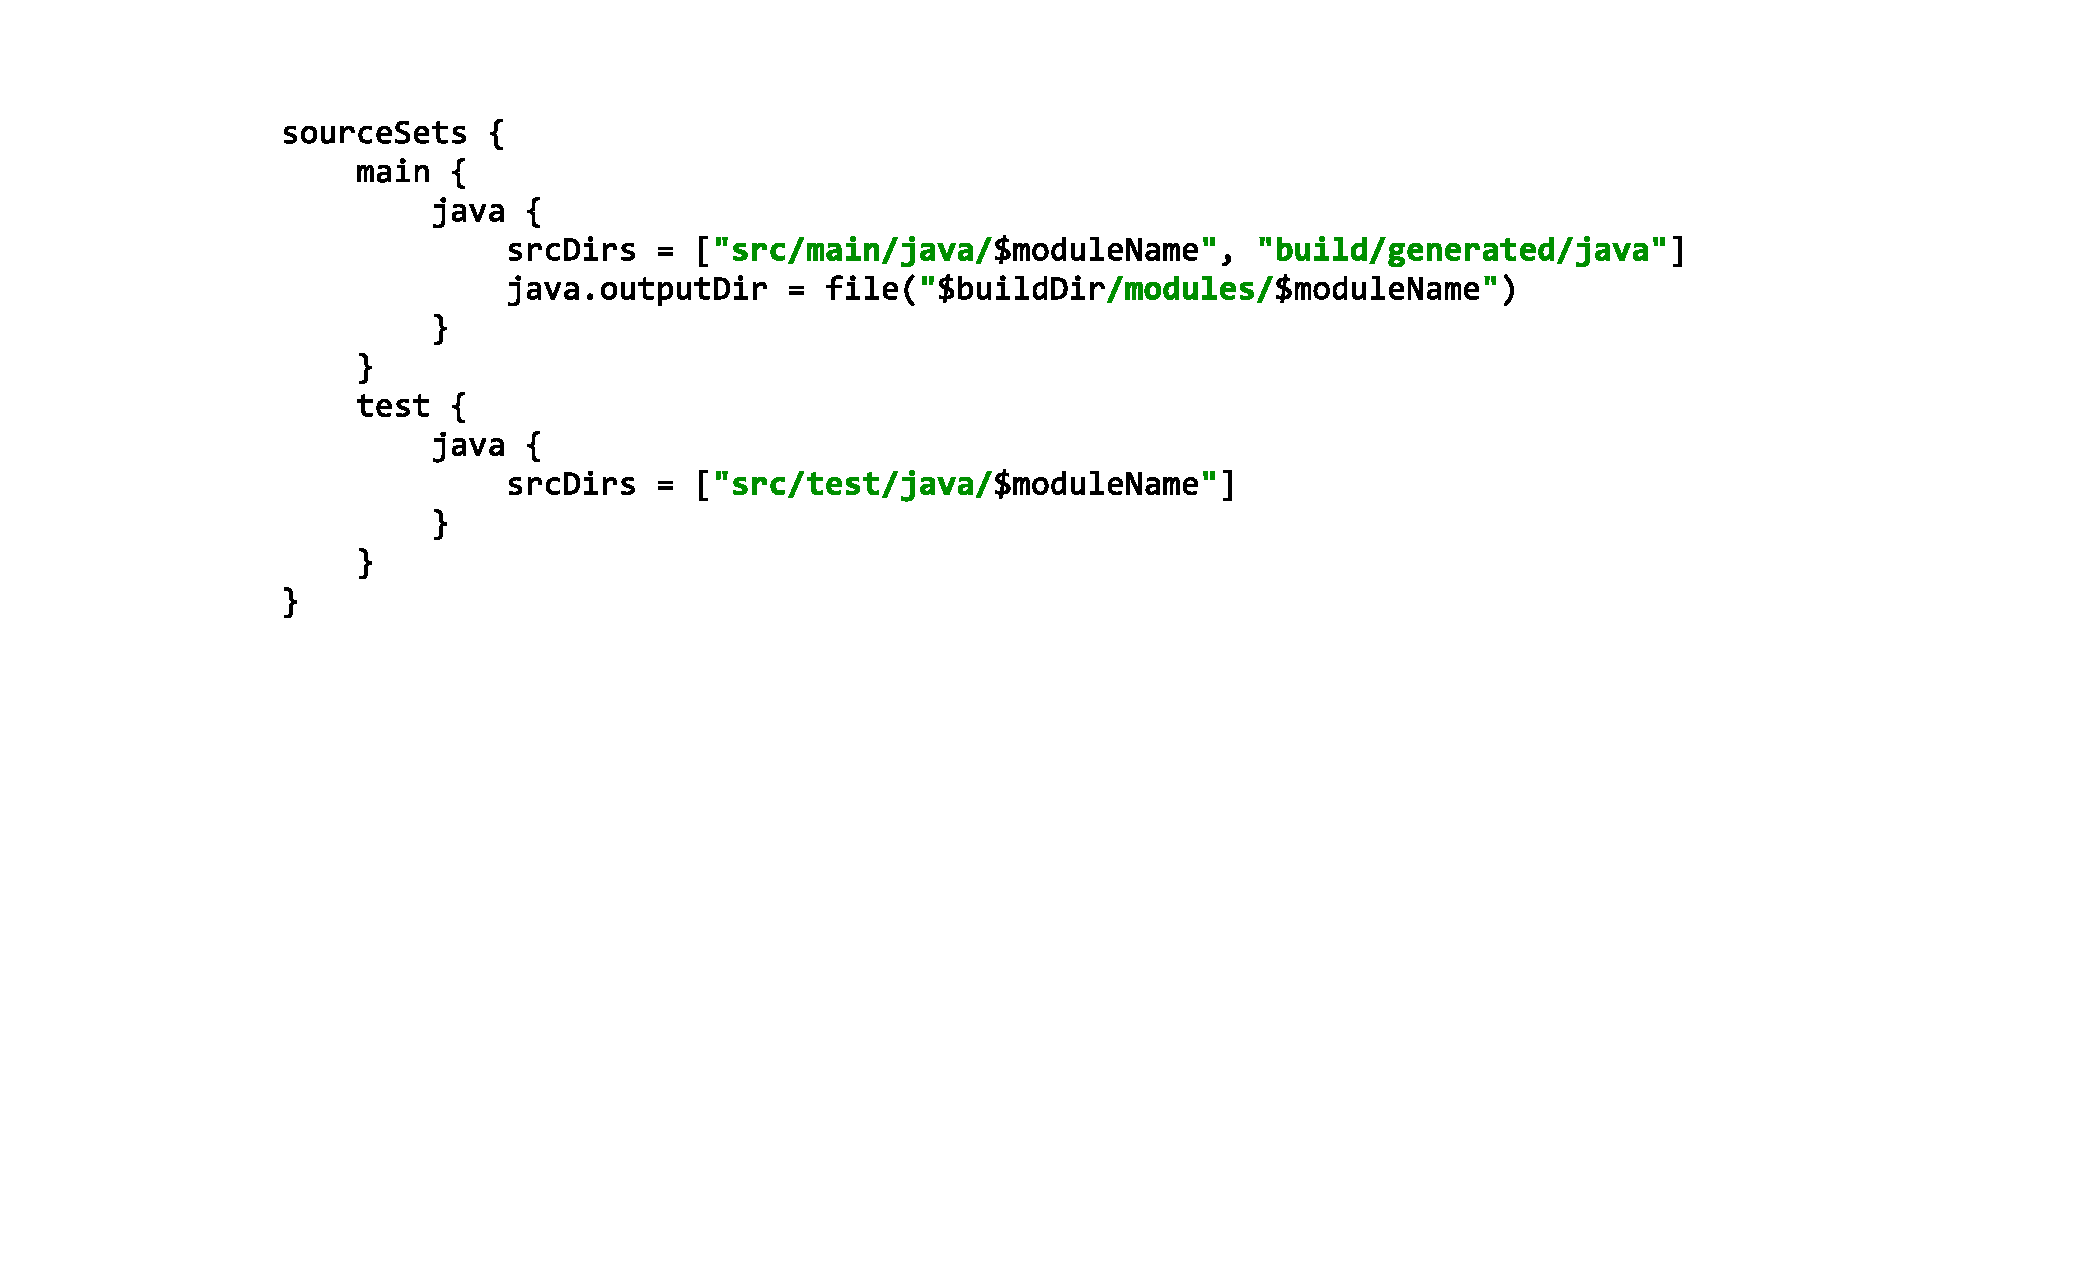
\includegraphics[width=0.7\textwidth]{material/images/sourcesets.pdf}
	  \caption{Source Sets}
	  \label{fig:Source_Sets}
	\end{figure}

 	Anschließend müssen die Java \textit{Source Sets} des Projekts bestimmt werden. Um die Umsetzung so einfach wie möglich zu gestalten, wird in der \textit{buld.gradle} Konfigurationsdatei, die für die Ausführungsphase zuständig ist, eine \textit{subprojects} Konfiguration angelegt, die für jedes Subprojekte die interne Projektstruktur definieren lässt. Diese beschreibt den Ort, an dem sich  Verzeichnisse mit den Java Code und den dazugehörigen Ressourcen befinden sollen.\bigbreak

	\begin{figure}[h!]
	  \centering
	  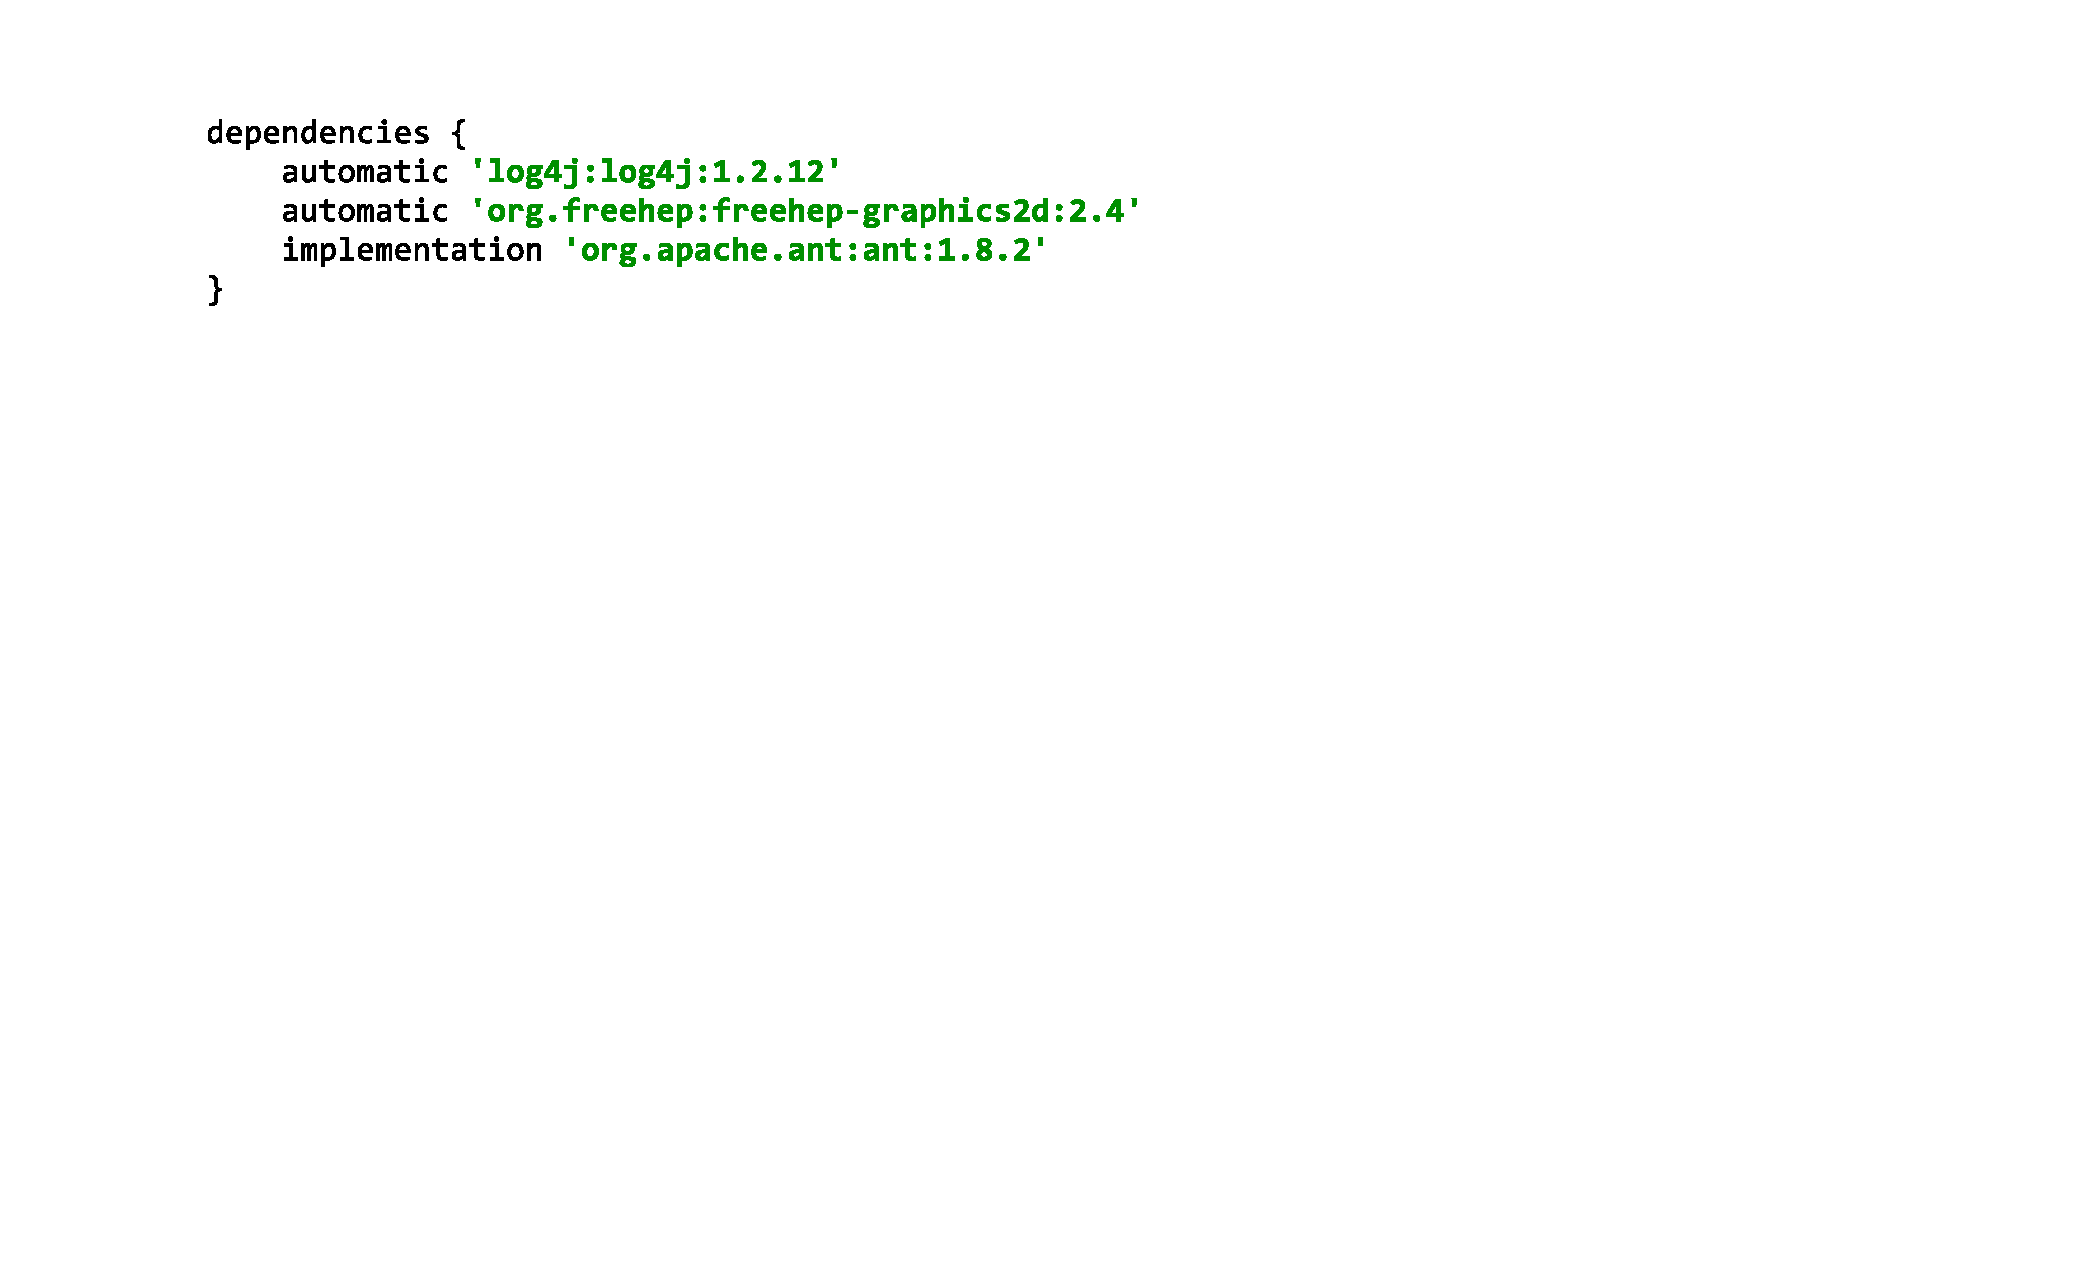
\includegraphics[width=0.6\textwidth]{material/images/gradle/dependencies.pdf}
	  \caption{Drittanbieter-Bibliotheken}
	  \label{fig:deps}
	\end{figure}

 	Im nächsten Schritt werden global genutzte Drittanbieter-Bibliotheken deklariert. Diese werden aus dem \textit{Maven Repository} beim Initiiere des Projekts geladen und auf den Klassenpfad aller Plugin Projekte eingebunden. Somit liegt die Verwaltung der Bibliotheken und der dazugehörigen Version an den \textit{Maven Repository} und muss nicht mehr im \textit{GitLab Repository} bereitgestellt werden.\newline
 	Zusätzlich erleichtert die Deklaration der Drittanbieter-Bibliotheken, unter einer separaten Konfiguration, die Aufgabe der manuellen Erstellung der Klassenpfade und die Einbindung der Bibliotheken in der Entwicklungsumgebung, da die Konfiguration von der Entwicklungsumgebung automatisch aufgegriffen und auf das Projekt angewandt wird.\bigbreak

	\begin{figure}[h!]
	  \centering
	  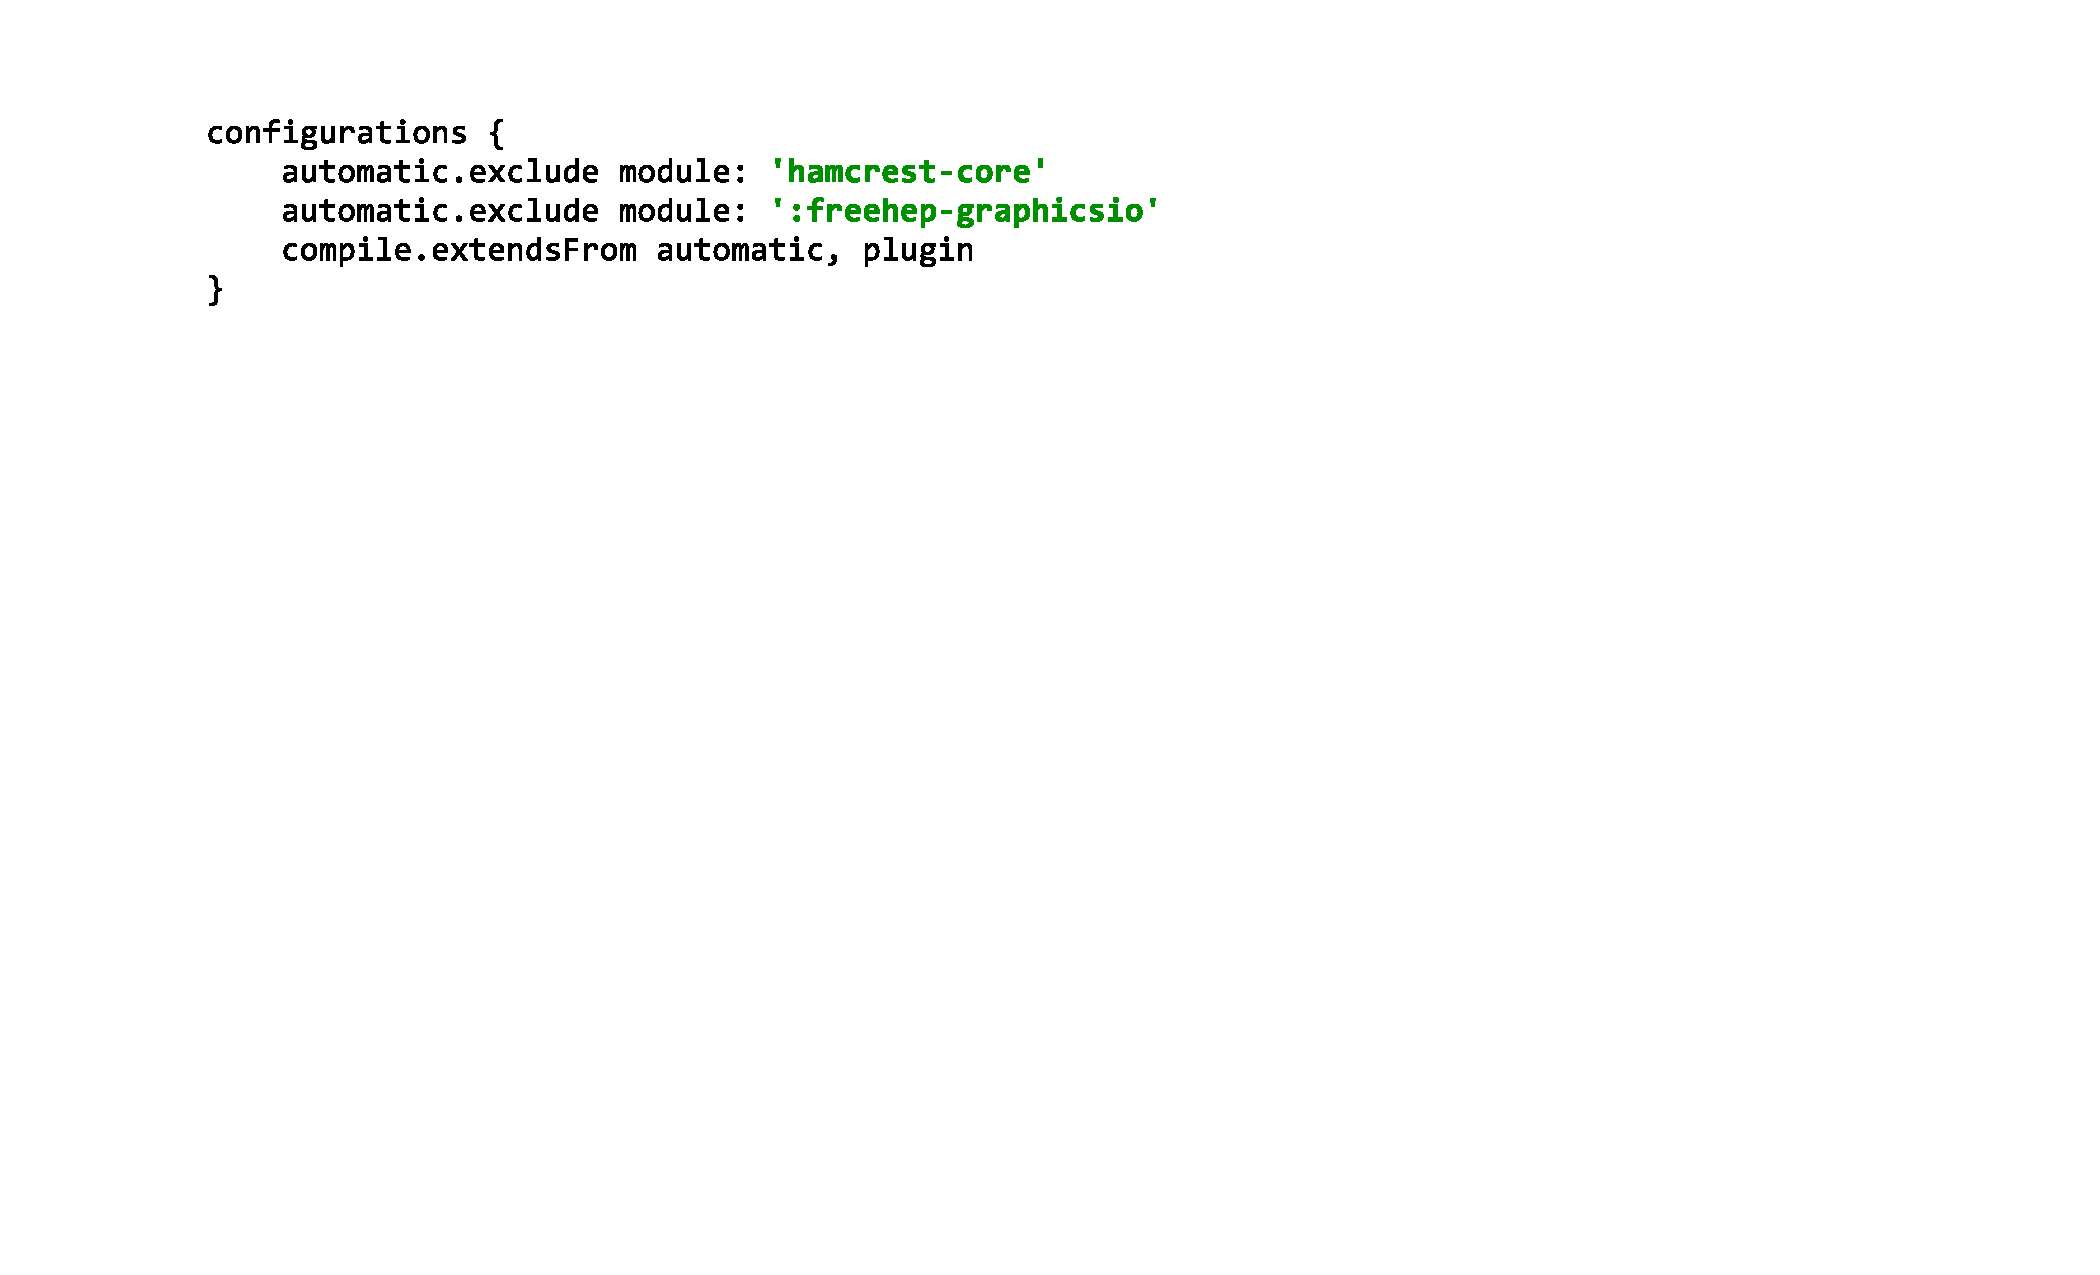
\includegraphics[width=0.6\textwidth]{material/images/gradle/configurations.pdf}
	  \caption{Klassenpfade}
	  \label{fig:kPath}
	\end{figure}

 	Um die Klassenpfade voneinander zu trennen, werden zusätzliche Konfigurationen mit dem Namen \textit{plugin} und \textit{automaitc} eingeführt, die Plugin Code und Drittanbieter-Bibliotheken voneinander trennen und für das Kompilieren zusammenführen. Somit können diese getrennt voneinander verwaltet, modifiziert und bei Bedarf für bestimmte Aufgaben angepasst werden.\bigbreak

	\begin{figure}[h!]
	  \centering
	  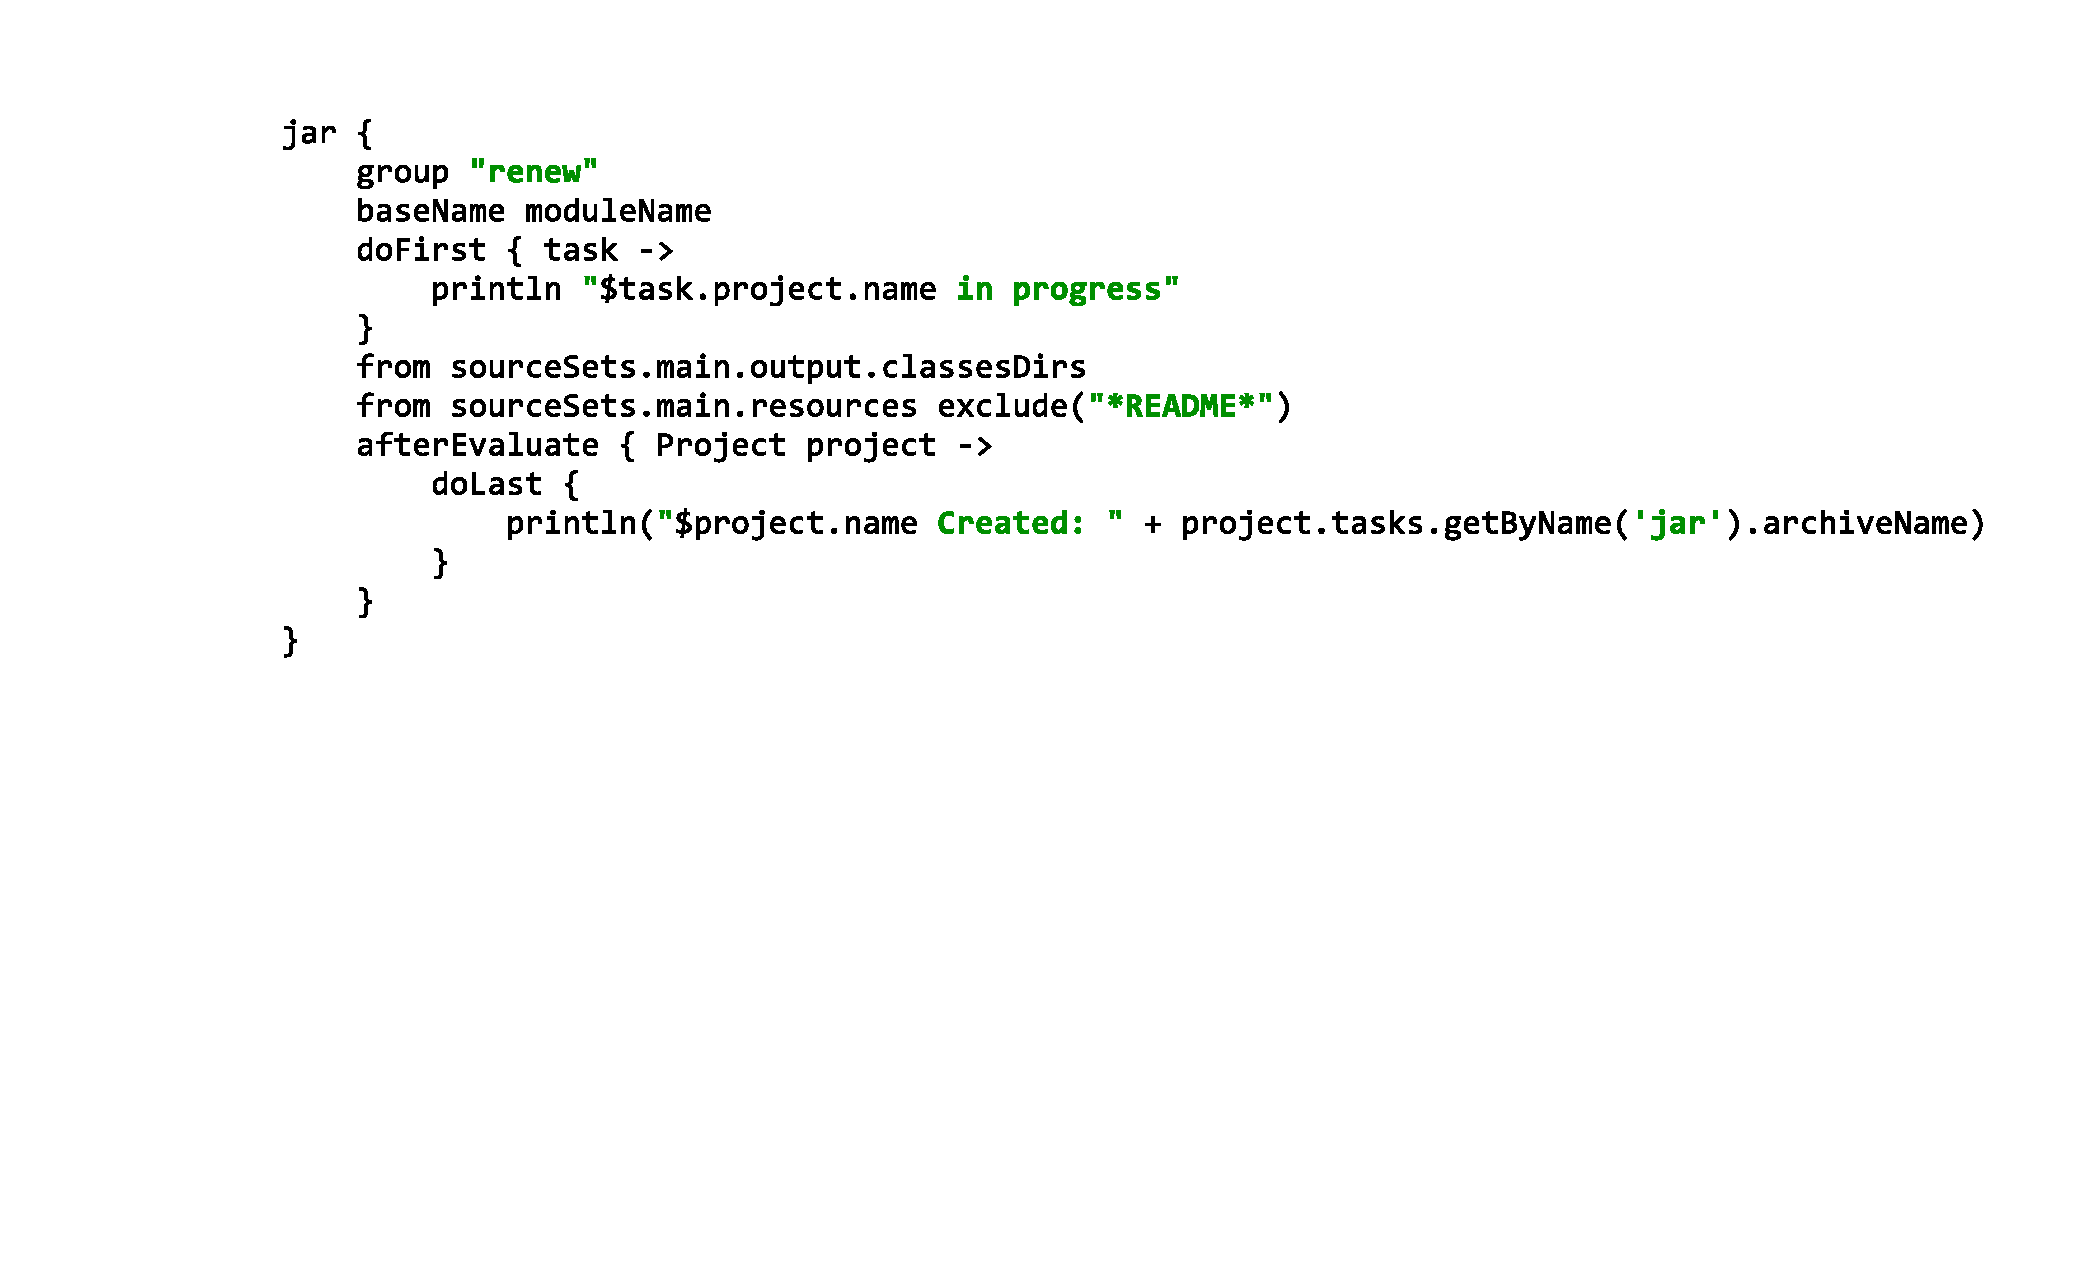
\includegraphics[width=\textwidth]{material/images/jar.pdf}
	  \caption{Jar Task}
	  \label{fig:jar}
	\end{figure}

	Zum Schluss der globalen Konfiguration wird ein \textit{jar} Task angelegt, der für ein gegebenes \textit{Source Set} ein \textit{jar}-Archiv für jedes Plugin mit den dazugehörigen Ressourcen erstellt.\newline
	Damit ist die globale Konfiguration der \textsc{Renew} Plugins beendet und bereit für die individuelle Anpassung der Plugin Bedürfnisse.\bigbreak

	\begin{figure}[h!]
	  \centering
	  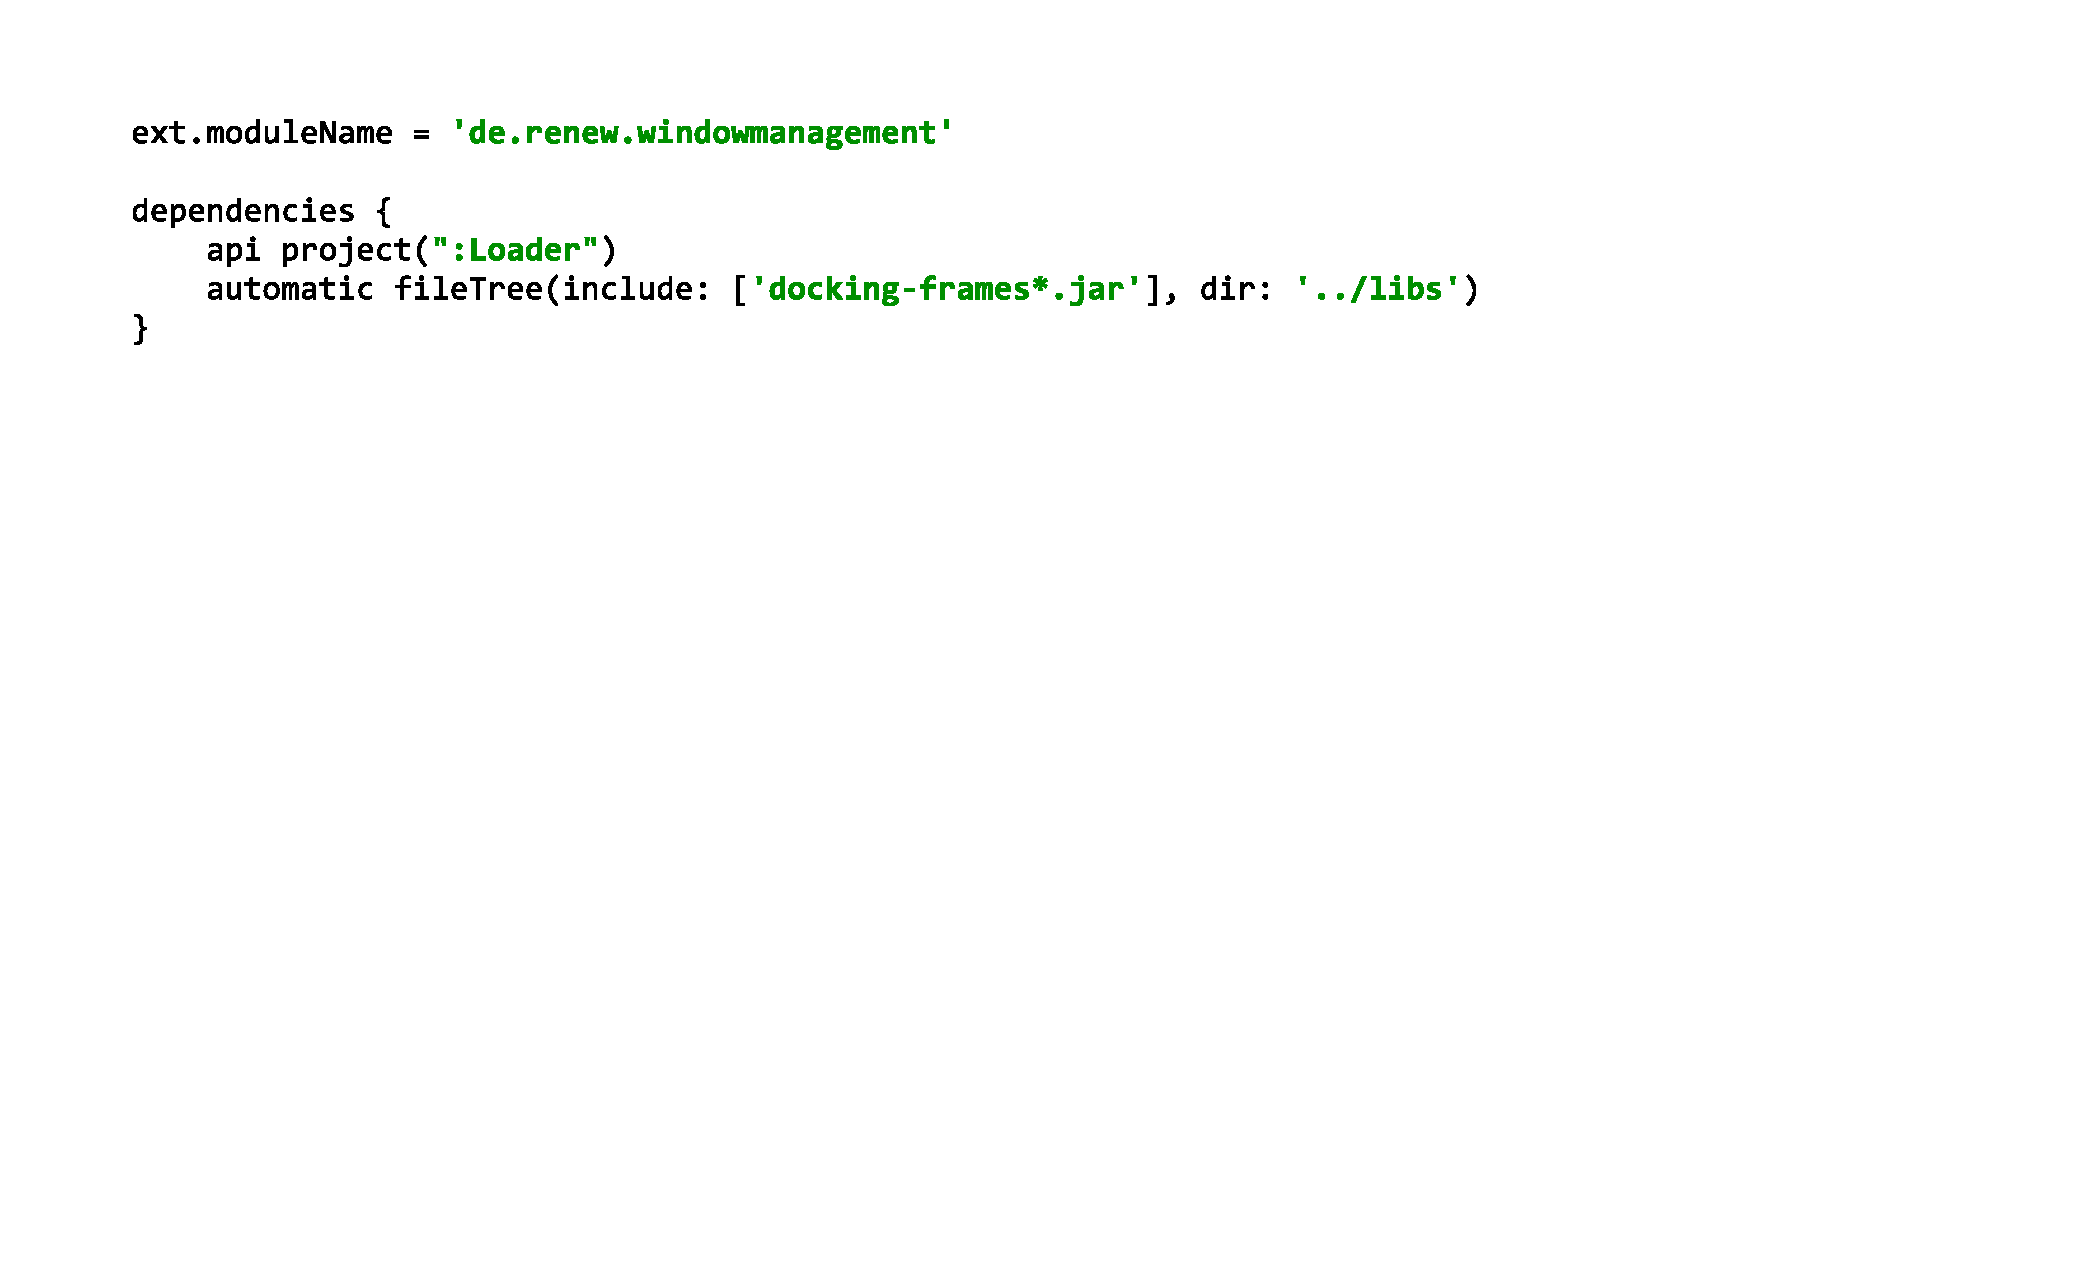
\includegraphics[width=0.8\textwidth]{material/images/gradle/winmangradle.pdf}
	  \caption{Individuelle Konfiguration}
	  \label{fig:windmang}
	\end{figure}

	Jedes einzelne Plugin benötigt einen internen Namen für die Verwaltung und die zusätzlichen Drittanbieter-Bibliotheken sowie Plugin Abhängigkeiten. Dafür wird in der Plugin \textit{buidl.gradle} Konfigurationsdatei der Name unter den \textit{extension properties} deklariert und die bereits geerbten Abhängigkeiten erweitert. In der Abbildung \ref{fig:windmang} wird das WindowManagment Plugin durch eine lokale, modifizierte Drittanbieter-Bibliotheken und durch das Plugin Projekt erweitert, um alle Benötigen Abhängigkeiten abzudecken.\bigbreak

	\begin{figure}[h!]
	  \centering
	  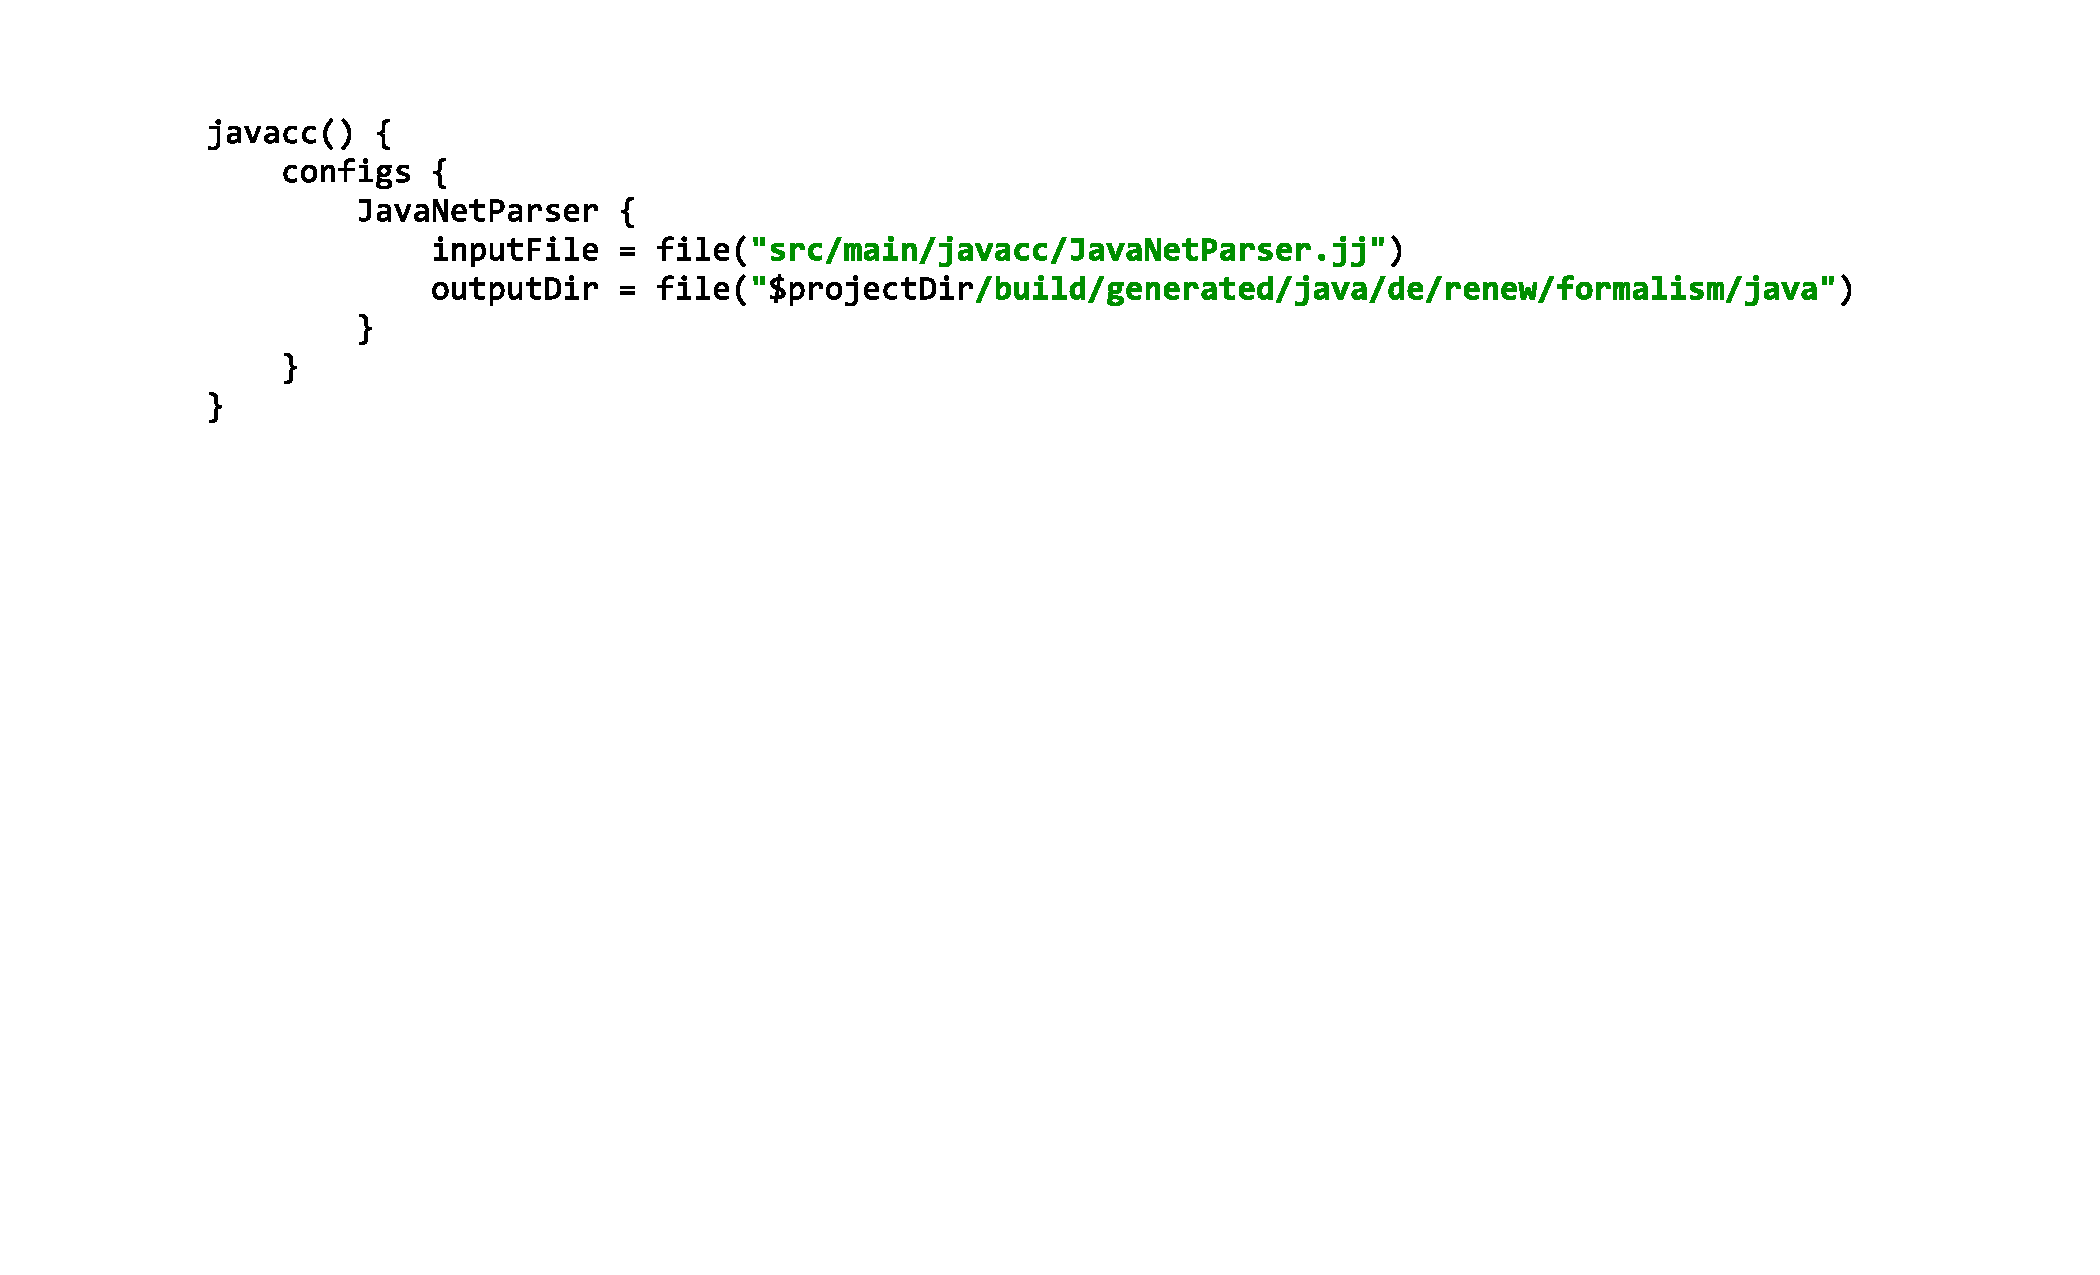
\includegraphics[width=\textwidth]{material/images/gradle/javacc.pdf}
	  \caption{Java Compiler Compiler}
	  \label{fig:javacc}
	\end{figure}

	Für die Konfiguration der einzelnen Plugins spielt der \textit{JavaCC} Parser eine große Rolle, denn dieser wandelt eine Grammatikspezifikation in ausführbaren Java Code um. Die genannte Technik wird in dem \textit{Formalism}, \textit{Feature Structures}, \textit{CH} und in dem \textit{Misc} Plugin verwendet. Der \textit{JavaCC} Parser erstellt Java Klassen, die obligatorisch für die Ausführung von \textsc{Renew} sind. Dementsprechend werden diese als generierte Ressourcen im \textit{build} Verzeichnis abgelegt und dem Java \textit{SourceSet} beigefügt. \bigbreak

	Jedes einzelne Plugin wird auf diese Weise konfiguriert und enthält einen Namen sowie zusätzliche Abhängigkeiten. Hiermit ist die Vorbereitung für die Modularisierung abgeschlossen. 


\subsection{Modularisierung}	
	Nachdem alle benötigen \textsc{Renew} Plugins kompiliert, verpackt und ausgeführt werden können, müssen die neu entstandenen Abhängigkeitsbeziehungen analysiert werden. Die Analyse der Plugins geschieht nun über die erstellten Gradle Scripte, die für jedes Projekt die benötigten Bibliotheken und Projekte für die Kompilation deklarieren. Aus diesen wird anschließend ein Abhängigkeitsgraph erstellt, der Zyklen und versteckte Abhängigkeiten offenlegt. \bigbreak

	\begin{figure}[h!]
	  \centering
	  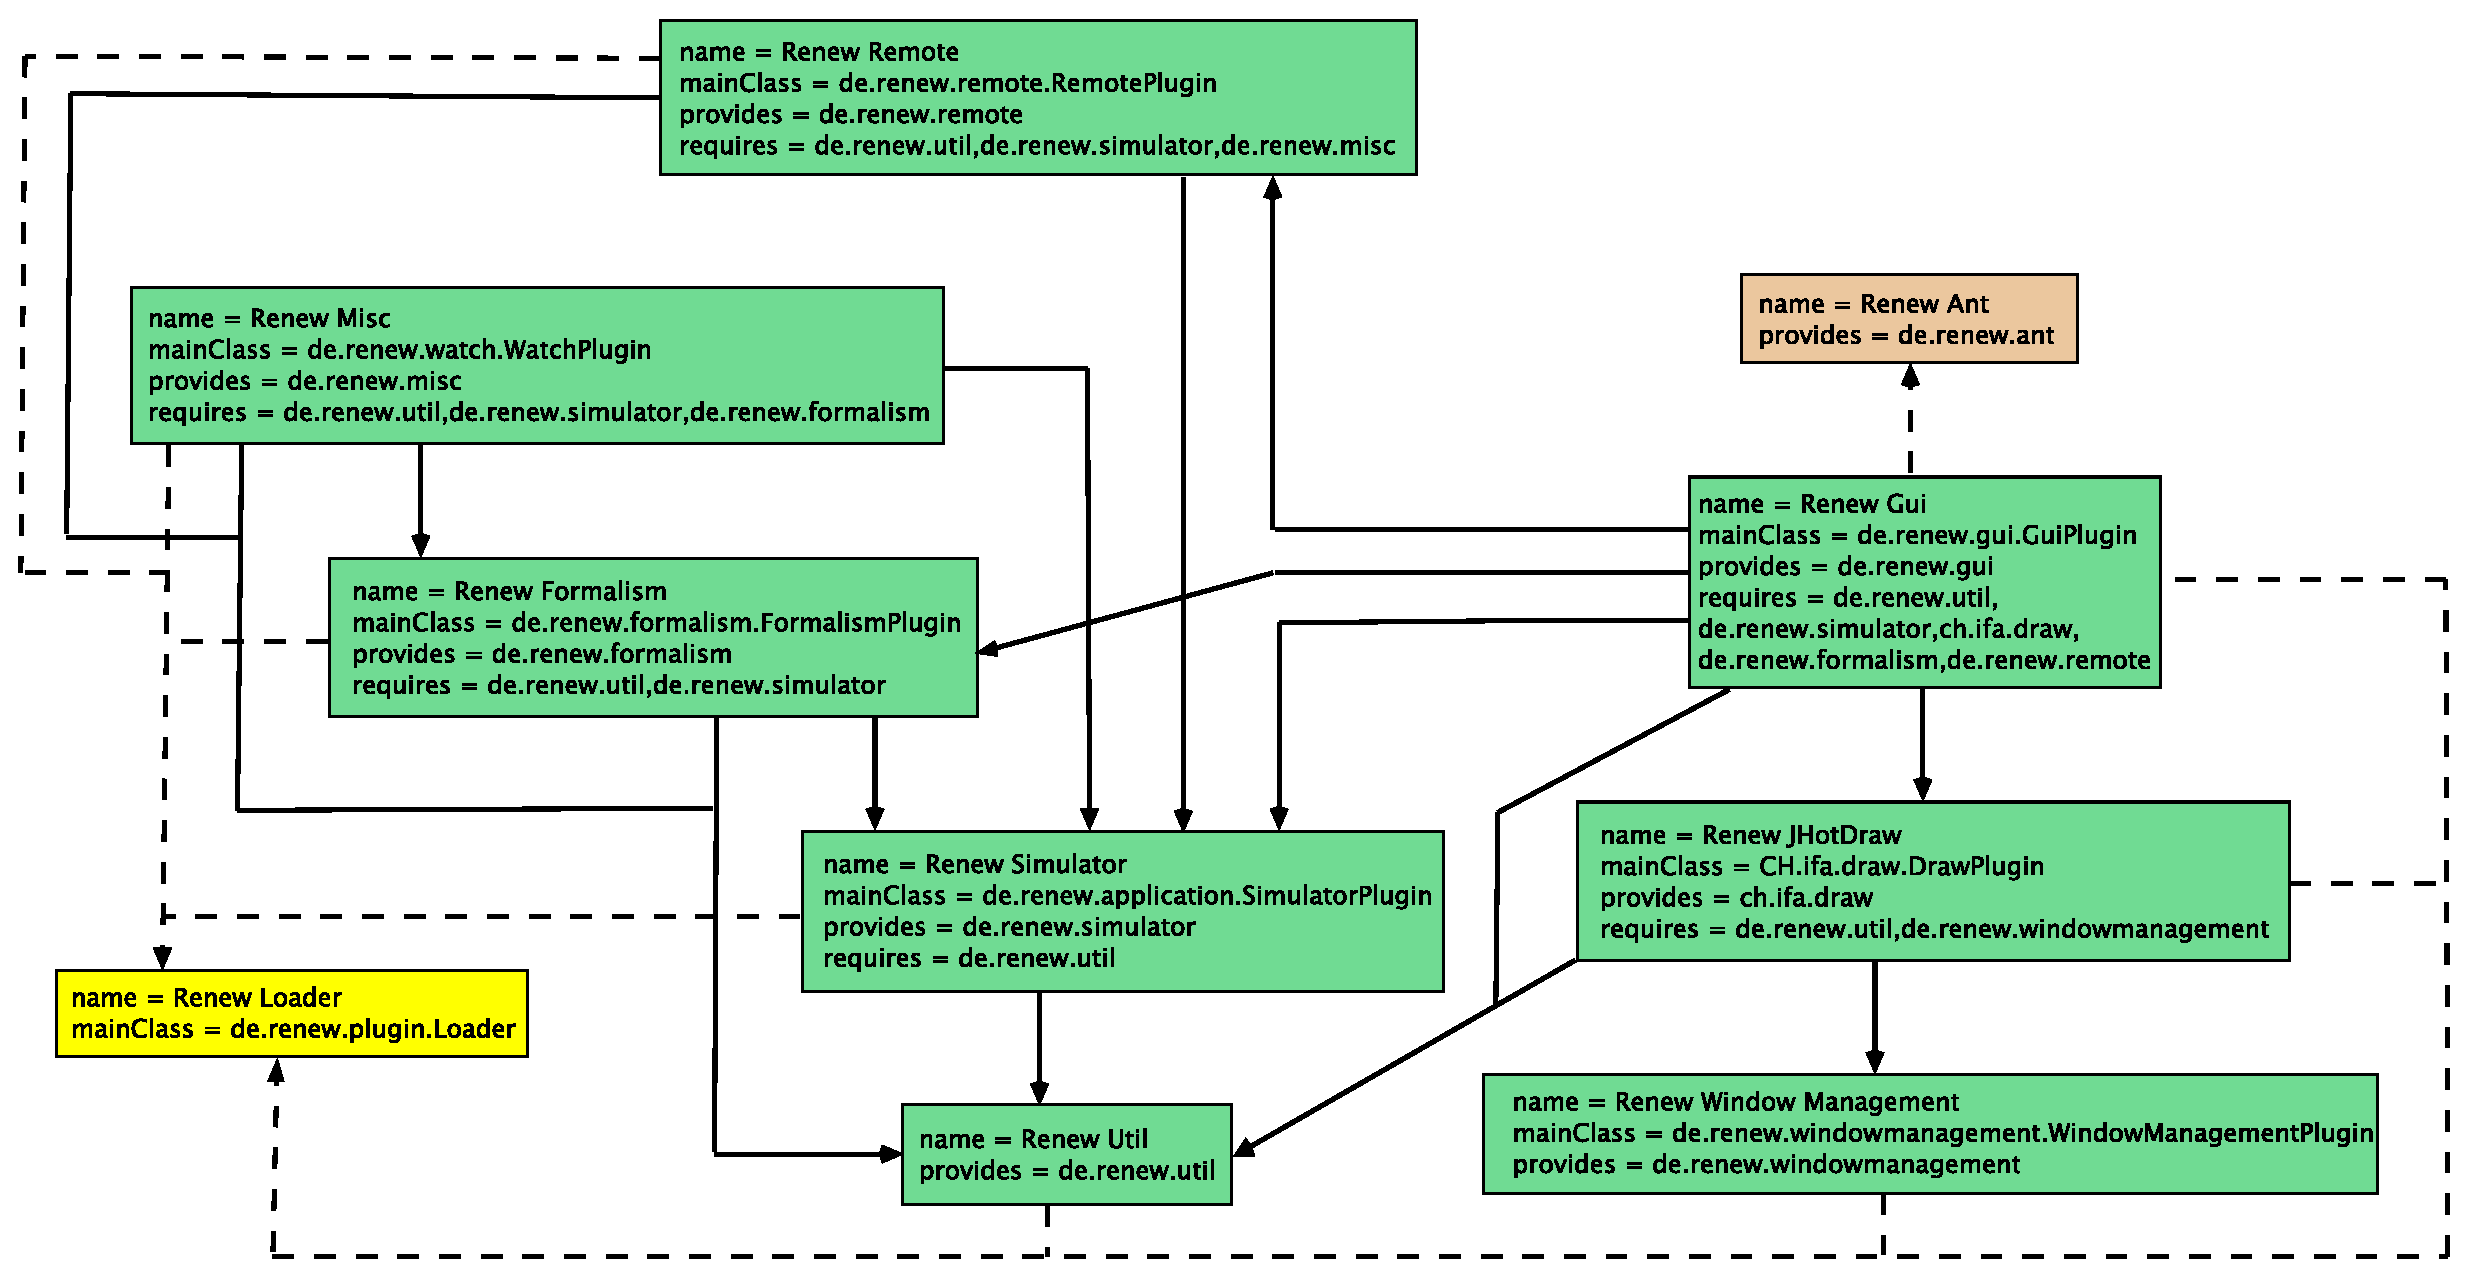
\includegraphics[width=\textwidth]{material/images/renew_plugin_dependencies-module-info.pdf}
	  \caption{Kompilation Abhängigkeiten}
	  \label{fig:mod_deps}
	\end{figure}

	Der neu entstandene Graf wurde im Vergleich zu dem Grafen aus der Ausgangssituation Abschnitt \ref{fig:plugin_deps} durch ein Plugin erweitert und bindet alle Plugins an das \textit{Loader} Projekt. Des Weiteren sind auf der Abbildung \ref{fig:mod_deps} keine Zyklen in der minimalen Version zu beobachten und dementsprechend müssen auch keine weiteren Anpassungen durchgeführt werden. \bigbreak

	Die Migration von der minimalen Version von \textsc{Renew} wird von den \textit{Loader, Util} und \textit{Windowmanagment} Plugin eingeleitet. Diese besitzen keine Abhängigkeiten innerhalb der Plugin Menge und brauchen keinen Zugriff auf den Klassenpfad nachdem sie sich auf dem Modulpfad befinden. Im Gegensatz dazu, behalten Plugins, die sich auf dem Klassenpfad befinden und als ein unbenanntes Modul interpretiert werden, alle Zugriffsrechte auf die interne Struktur migrierter Plugins, wie bereits in den Abschnitt \ref{fig:modacc} beschrieben wurde.\bigbreak

	Da ein Modul seine eigene Abhängigkeiten verwalten muss, wird für jedes Plugin eine \textit{module-info.java} Konfigurationsdatei angelegt, die alle Java internen sowie Drittanbieter Bibliotheken auflistet. Für die ersten Module werden die erforderlichen Bibliotheken inklusive dem Loader Plugin in der Konfigurationsdatei mit dem Schlüssel \textit{requires} verankert und die dazugehörigen Drittanbieter-Bibliotheken aus dem Klassenpfad auf dem Modulpfad als automatische Module aufgesetzt.

	\begin{figure}[h!]
	  \centering
	  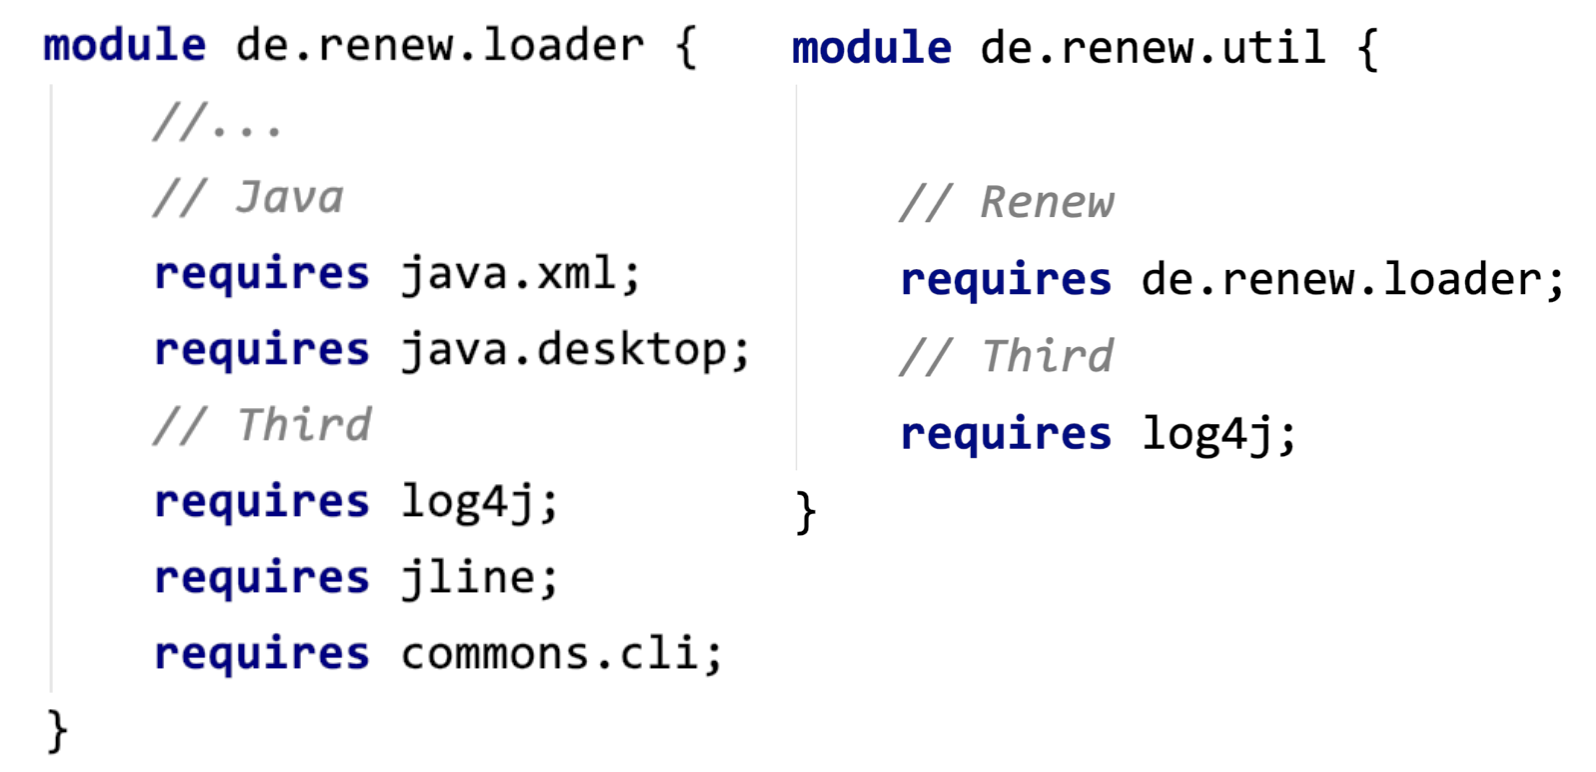
\includegraphics[width=0.7\textwidth]{material/images/loaderUtil-info.png}
	  \caption{Benötigten Bibliotheken}
	  \label{fig:loaderUtil}
	\end{figure}

	In diesem Zustand wird \textsc{Renew} kompiliert und ausgeführt. Das Ergebnis ist eine lauffähige Applikation, die ihre vollständige Funktion zugleich aus dem Modul- und Klassenpfad bezieht und identisch zu der initialen minimalen Version von \textsc{Renew} funktioniert.\newline
	Im nächsten Schritt werden Plugins migriert, die nur auf die neu entstandenen Module aufsetzen, wie zum Beispiel das \textit{Simulator} und das \textit{JHotDrow} Plugins. Ihre Abhängigkeiten liegen auf dem Modulpfaden, daher gibt es keinen Grund mit dem Klassenpfad zu interagieren. \newline
	Da diese die zweite Modulschicht repräsentieren, fordern sie bestimmte Funktionalität mit dem \textit{requiers} Schlüssel aus den Loader, Util und Windowmanagment Plugins. Um dieser Anforderung zu entsprechen, müssen die notwendigen Plugins ihre Pakete  explizit für ihre Nutzer öffnen. Dazu deklarieren die angeforderten Plugins in ihrer \textit{module-info.java} mit dem \textit{exports} Schlüssel Pakte, die sie für andere Plugins zur Verfügung stellen möchte.

	\begin{figure}[h!]
	  \centering
	  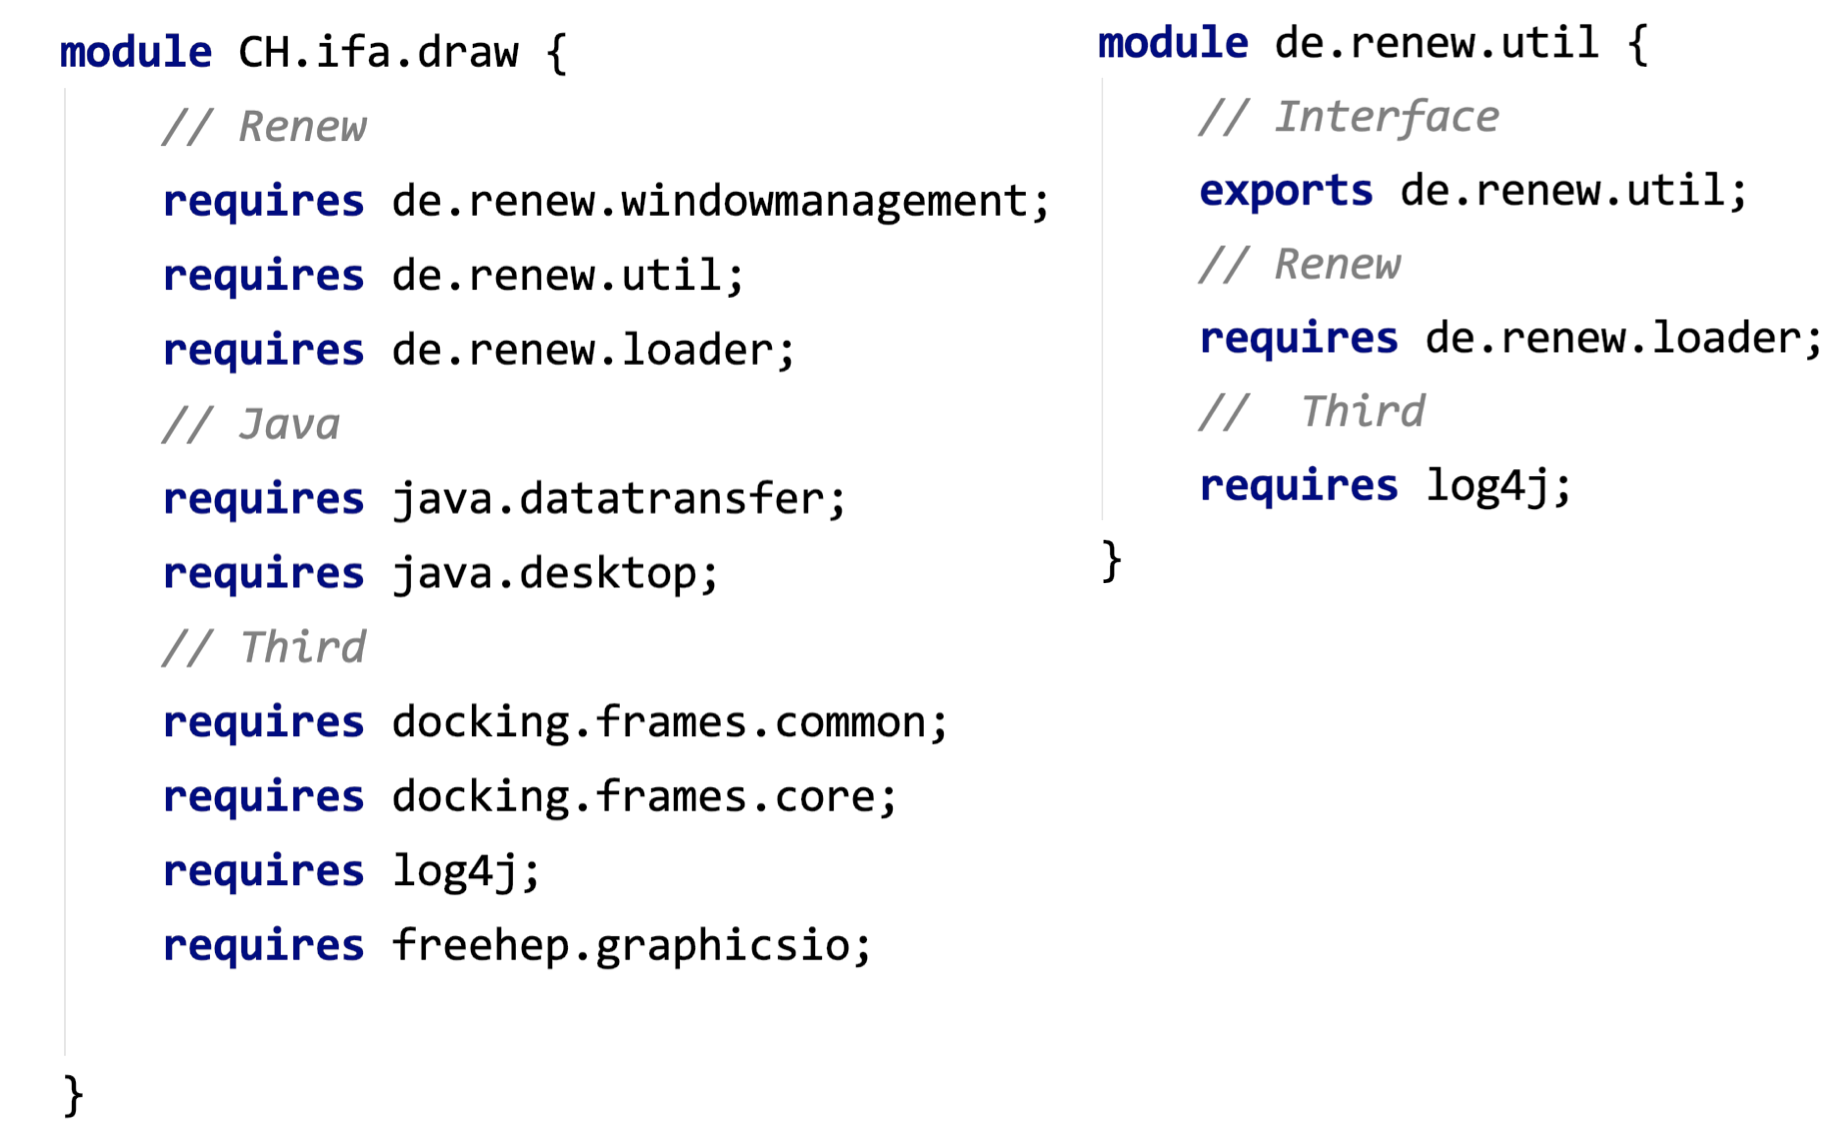
\includegraphics[width=0.7\textwidth]{material/images/utilCH-info.png}
	  \caption{Exportierte Pakete}
	  \label{fig:utilCH}
	\end{figure}

	In der Abbildung \ref{fig:utilCH} wurde das Util Plugin Modul angepasst und bietet jetzt das \textit{de.renew.util} Paket für den Gebrauch an.\newline
	Die Adaption der bestehenden Module muss mit jeder neuen Modulschicht an die angeforderten Pakete und Klassen angepasst werden, bis alle Abhängigkeiten erfüllt sind.\newline
	Damit sind die notwendigen Schritte für die Modularisierung bestimmt worden und können in einem Zyklus, bis sich alle Plugins auf dem Modulpfaden befinden, durchgeführt werden. Nämlich das Auslesen und Definieren der Plugin Kompilation- sowie Laufzeit Abhängigkeiten aus dem Gradle Build Skript mit dem Schlüssel \textit{requires} und das Nachrüsten der Schnittstellen bestehender Module mit dem \textit{exports} Schlüssel. \bigbreak

	In der folgenden Abbildung wird die komplette Migration in vier Schritten dargestellt. Zuerst wird das \textit{Loader}, das \textit{Utils} und das \textit{Window Management} Plugin migriert, da diese laut der Ausgangssituation keine Abhängigkeiten im Klassenpfad besitzen und nicht aus dem Modulpfad auf den Klassenpfad nicht zugreifen müssen. Im nächsten Schritt werden Plugins modularisiert, die nur auf den Modulpfad angewiesen sind. Das wären der \textit{Simulator} sowie \textit{JHotDraw} Plugin. Da alle Abhängigkeiten des \textit{Formalism} und \textit{Remote} Plugins auf den Modulpfad bewegt worden sind, können diese der Modulmenge beigefügt werden. Zum Schluss bleiben Plugins mit weit gefächerten Plugin Abhängigkeiten, wie zum Beispiel das \textit{Misc} oder das \textit{Gui} Plugin.  \bigbreak

	\begin{figure}[h!] 
	  \centering
	  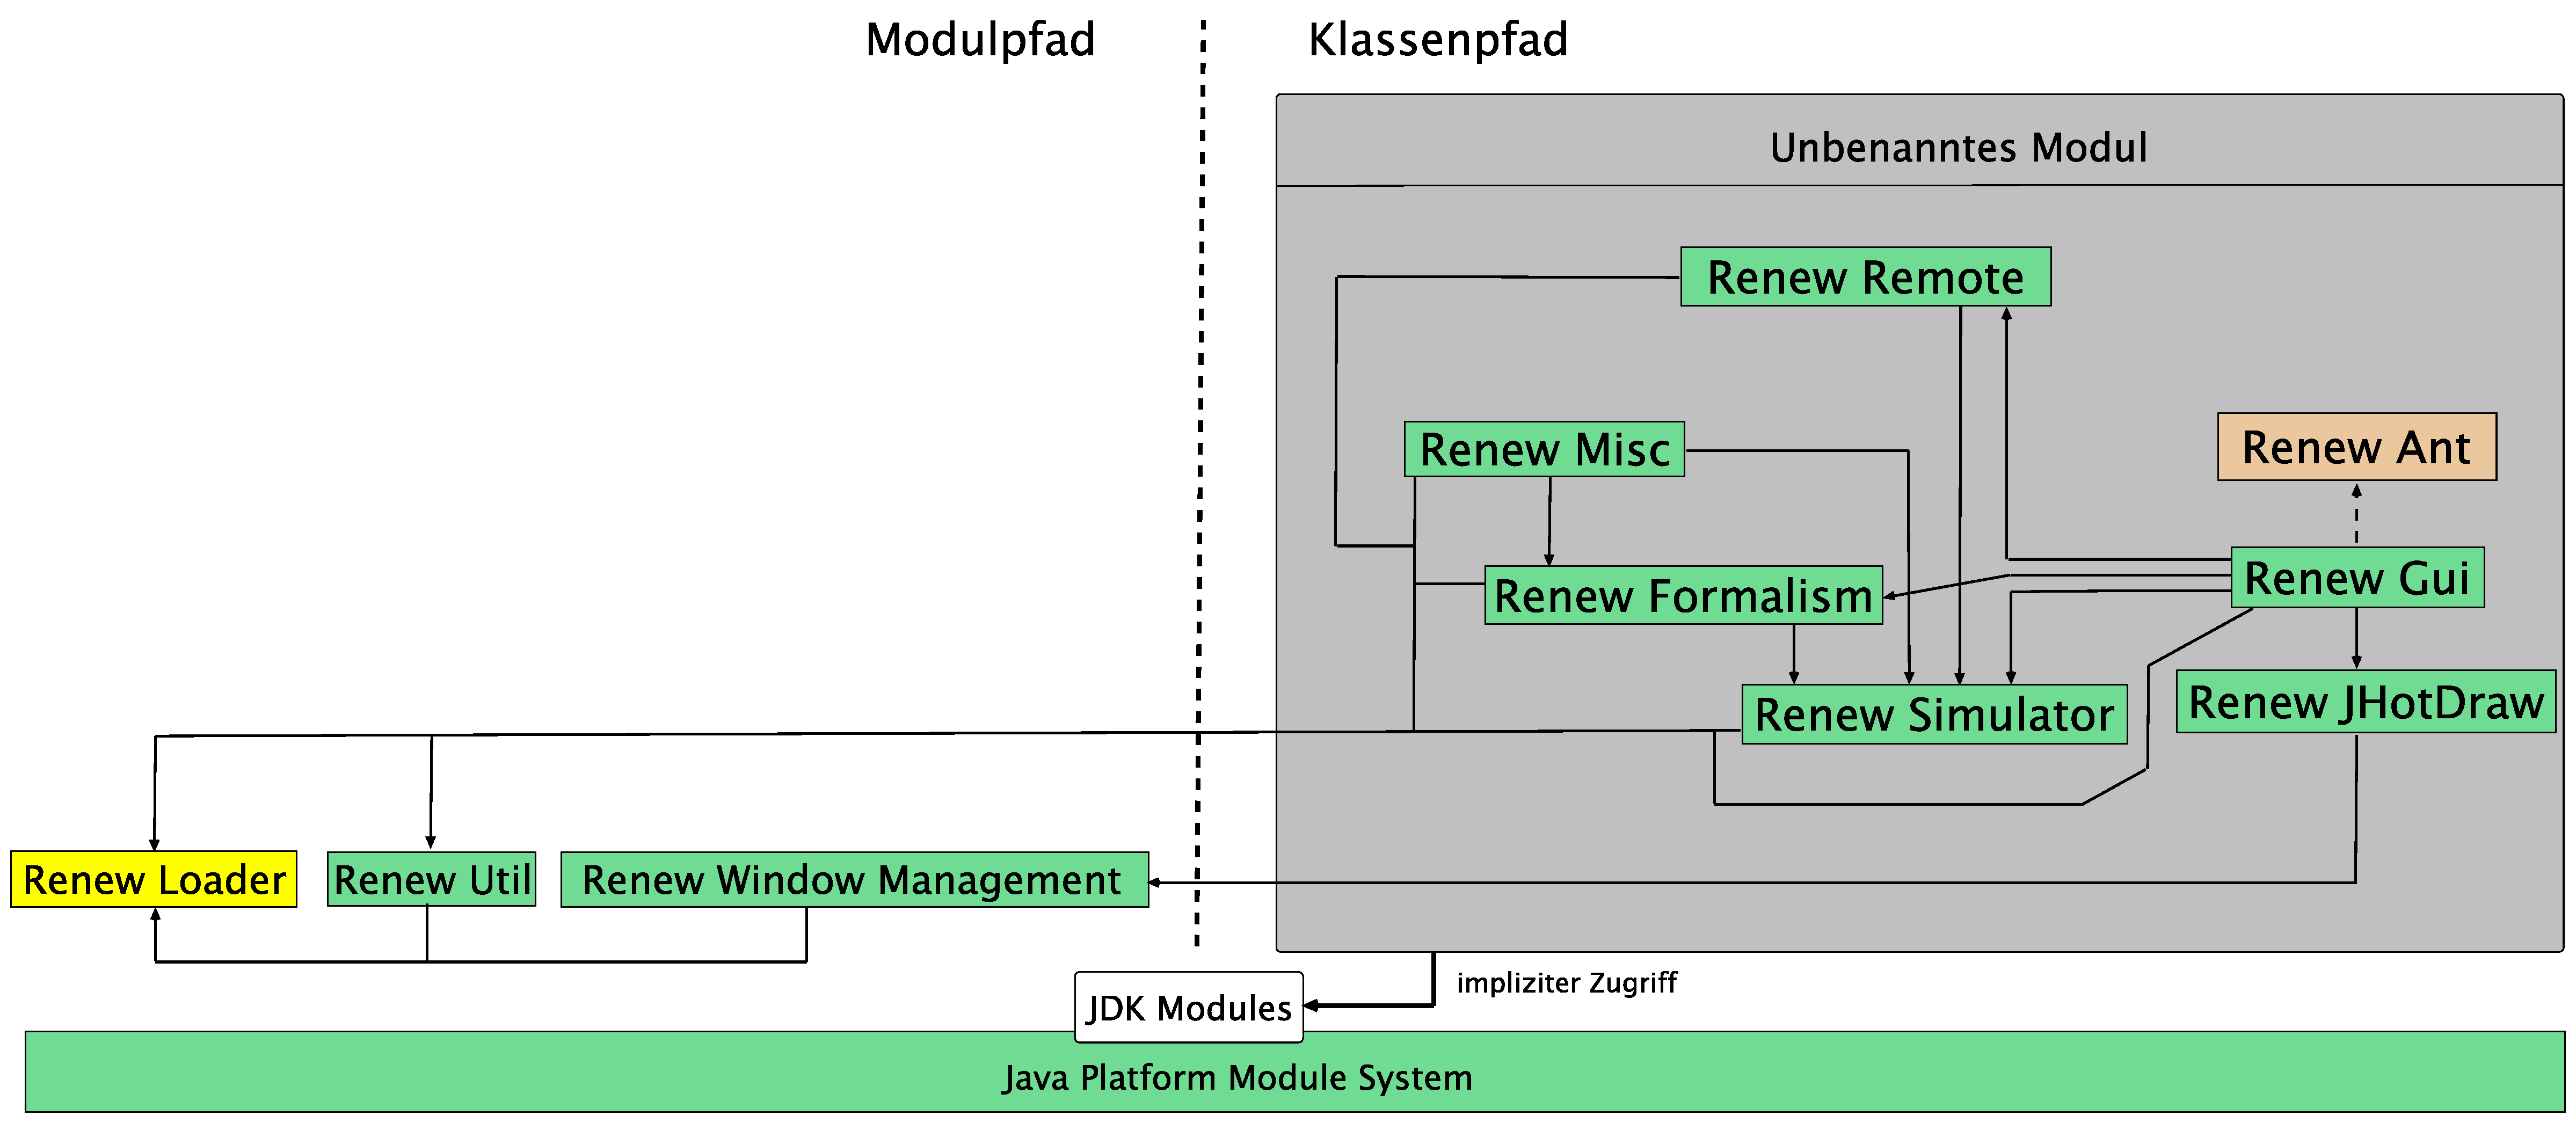
\includegraphics[width=0.997\textwidth]{material/images/renew_plugin_dependencies-migrate_1b.pdf}
	 \end{figure}
	\begin{figure}[h!] 
	  \centering
	  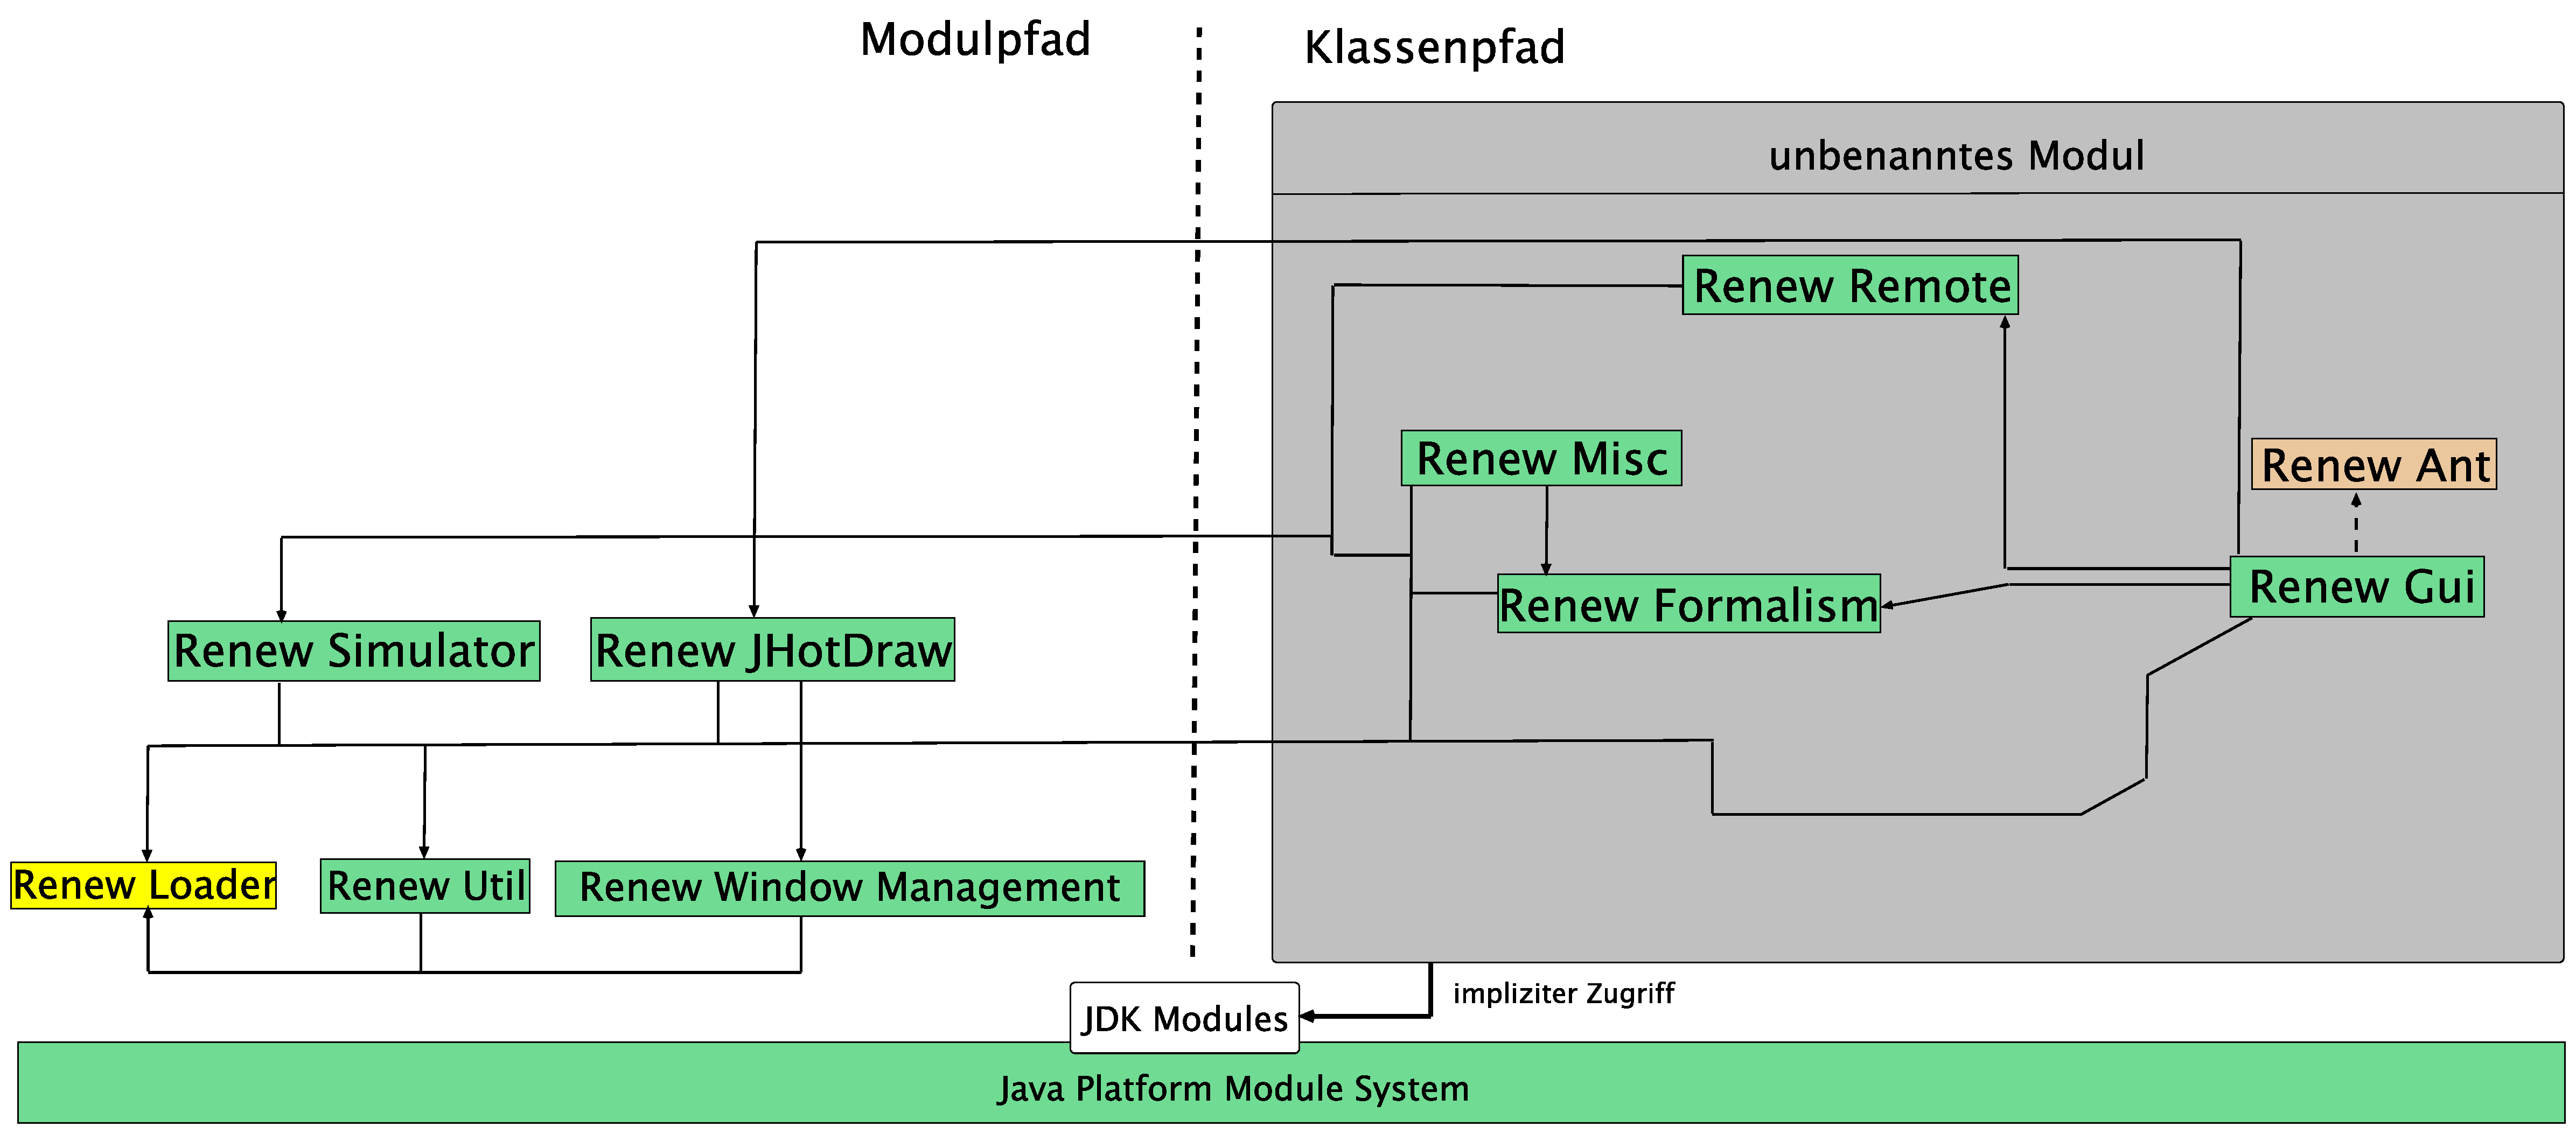
\includegraphics[width=0.997\textwidth]{material/images/renew_plugin_dependencies-migrate_2b.pdf}
	  \end{figure}
	 \begin{figure}[h!] 
	  \centering
  	  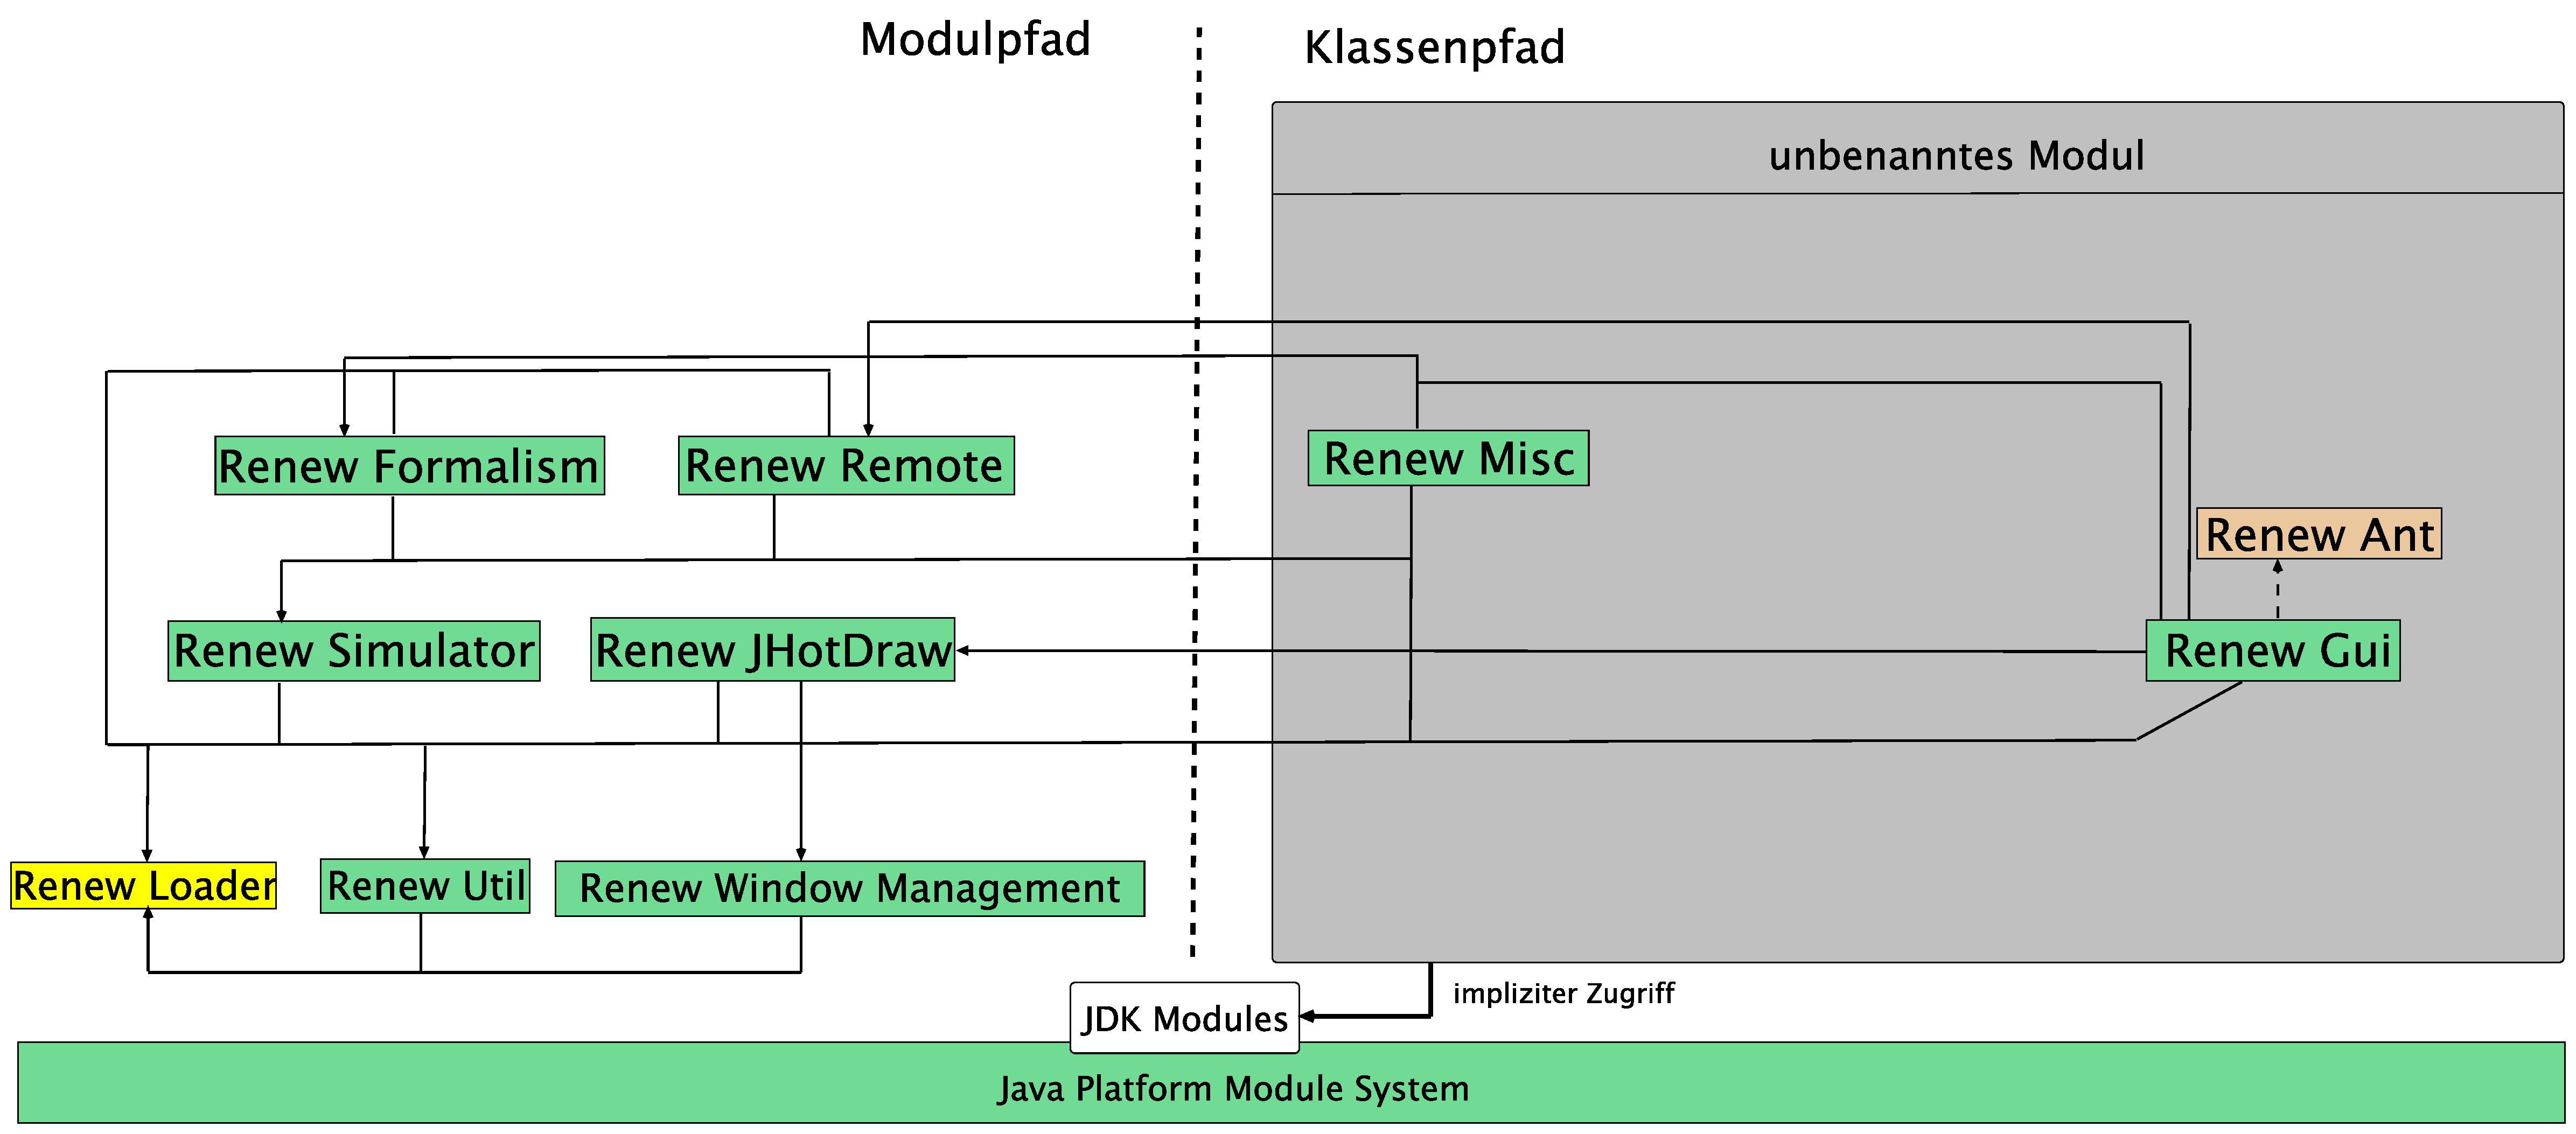
\includegraphics[width=0.997\textwidth]{material/images/renew_plugin_dependencies-migrate_3b.pdf}
  	  \end{figure}
  	 \begin{figure}[h!] 
	  \centering
  	  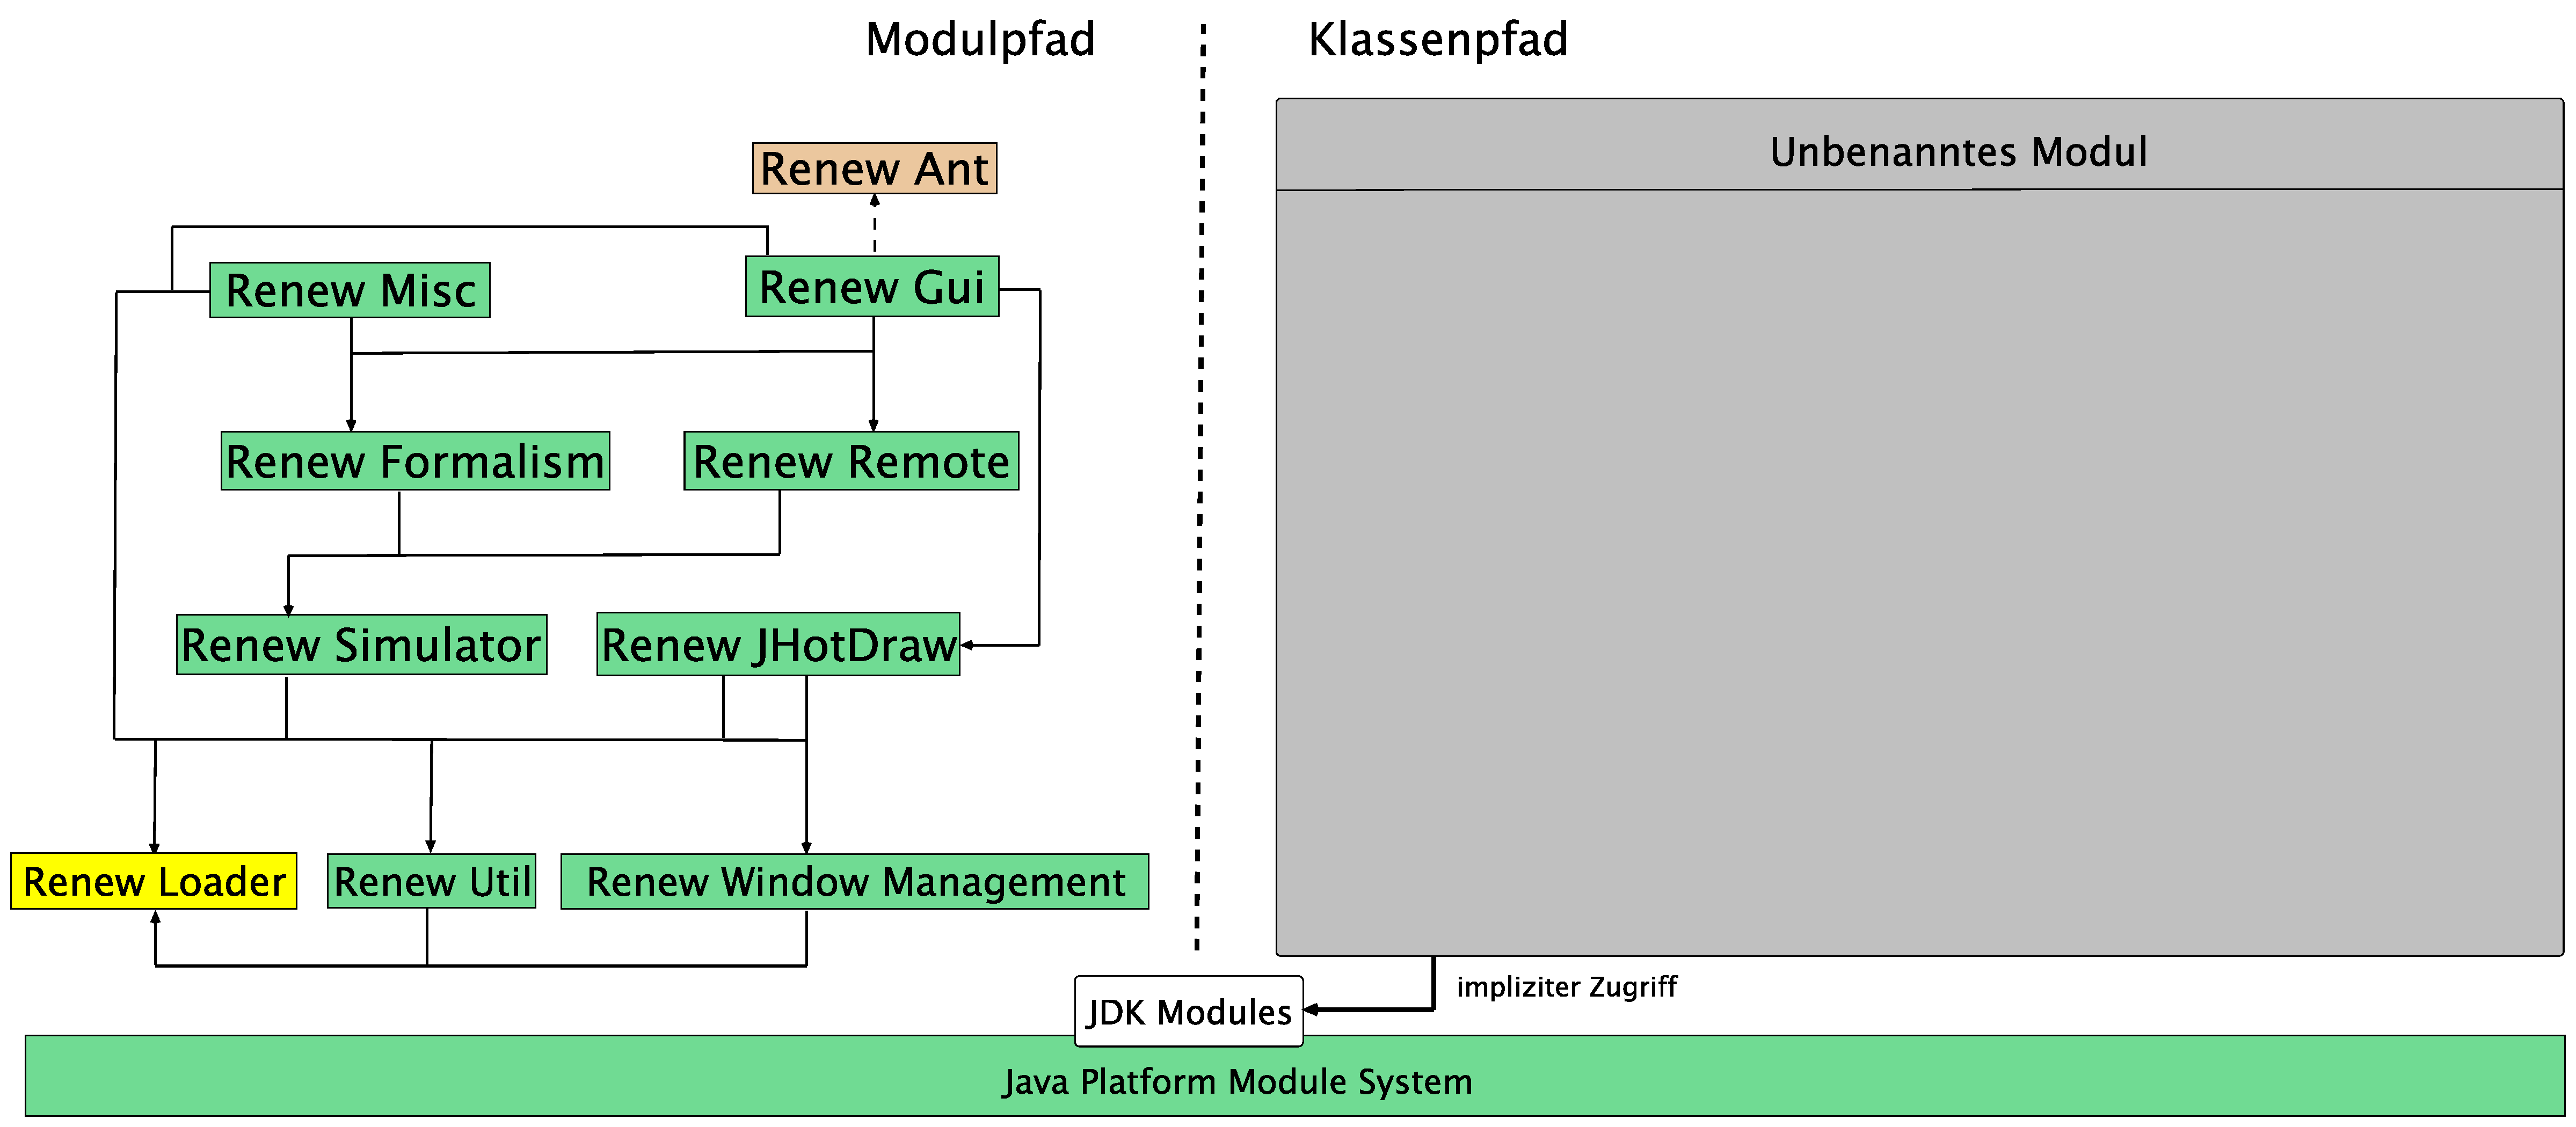
\includegraphics[width=0.997\textwidth]{material/images/renew_plugin_dependencies-migrate_4b.pdf}
  	  \caption{Migration}
	  \label{fig:mig}
	\end{figure}

\newpage
\section{Evaluation}
	Die Evaluation des ersten Prototyps bewertet das Ergebnis des gesetzten Ziels, nämlich die Erstellung einer minimalen \textsc{Renew} Version für das Modulsystem von Java. Dafür werden die Schlüsselaktionen der Migration wie Projektstruktur, Projektverwaltung und die Modulumsetzung nacheinander kritisch beleuchtet.

\subsection{Struktur} \label{sub:struktur}
	Die Anforderung eine minimalen Version von \textsc{Renew} zu modularisieren und mit einem modernen Werkzeug zu verwalten wurde erfüllt. Diese Aufgabe beinhaltete das Umstrukturieren der Plugin Code Basis, die es erlaubt zusätzliche Module innerhalb eines Plugins anzulegen. Jedoch gab es unerwartete Strukturänderungen, die durchgeführt werden müssen. Zum Beispiel besitzen einige Plugins wie das Util, Loader und Simulator Plugin Test Klassen, die in die neue Struktur eingebunden werden müssen. Demzufolge musste laut dem Maven Standard Layout ein \textit{src/test/java/module.name} Test Ressourcen, mit den dazugehörigen Test Klassen, angelegt und verwaltet werden. \newline

	Des Weiteren werden JavaCC Klassen separat von den Java Ressourcen untergebracht und von einem Gradle Plugin ausgeführt. Dies hat zur Folge, dass der generierte Code umgeleitet werden muss, um an der entsprechenden Position die Funktion zu erfüllen. Zusätzlich muss JavaCC den Java Code generieren, bevor der Java Compiler mit der Übersetzung beginnt, denn die generierten Java Klassen bilden die Basis für die Plugins und somit sind sie zwingend erforderlich für die Kompilation. Dies bezüglich wurde der \textit{Gradle Task Graph} modifiziert, um die entsprechende Reihenfolge zu erfüllen. Daraus ergibt sich eine Komplexität, die neu für \textsc{Renew} ist und in der Zukunft sorgfältig gewartet werden muss. \bigbreak

\subsection{Verwaltung} \label{sub:verwaltung}
	Ein wesentlicher Vorteil der modernen \textit{build} Tools wie Gradle und Maven, ist die Verwaltung der verwendeten Drittanbieter-Bibliotheken. Diese laden und binden benötigte Bibliotheken mit dem kompletten Abhängigkeitsgraphen in das Projekt ein, ohne den Zwang der Einarbeitung des Entwicklers in die Struktur der genutzten Bibliothek. Somit wird viel Zeit gespart, da man sich mit dem Kontext und den darunter liegenden Bausteinen, wie Core, Common und Util, der genutzten Bibliotheken nicht beschäftigen muss. \newline

	Die Verwaltung der Bibliotheken spielt eine große Rolle für Renew, da im Verlauf der Entwicklung, Drittanbieter-Bibliotheken angepasst wurden und somit keine Möglichkeit besteht eine saubere Version der Bibliothek einzubinden. Infolgedessen entstehen  unsaubere Abhängigkeiten, die nicht aktualisiert werden können. Diese werden wie zuvor durch das Auslesen aus einem lokalen \textit{libs} Verzeichnis in das Projekt eingebunden und müssen in der Zukunft für die saubere Umsetzung von der benutzerdefinierten Logik befreit werden.\bigbreak

	Ein zusätzlicher Vorteil der neuen Projektverwaltung liegt an der neuen Umsetzung mit einer Programmiersprache, die es erlaubt, mit Feldern, Variablen, Schleifen und Objekten zu arbeiten. Dies hat zur Folge, dass der Übergang von den \textsc{Renew} Java Code zu den \textit{build} Skript von Gradle für den Entwickler leichter nachzuvollziehen ist und somit Akzeptanz und Anpassungsfähigkeit mit sich bringt. \newline
	Hierzu kann die Verständlichkeit des Gradle Werkzeug gegenüber dem Ant Werkzeugs an der benötigten Code Menge, die geschrieben werden muss, verglichen werden. Zum Beispiel benötigt die Ant Version von Renew, die zurzeit alle Plugins und den kompletten Umfang der Applikation verpackt, um die 740 Zeilen für die globale Konfiguration und 135 Zeilen für jedes Projekt. Im Gegensatz dazu wiegt die minimale Gradle Version von \textsc{Renew} 136 Zeilen für die globale Konfiguration und nur 20 Zeilen für jedes Plugin im Durchschnitt. Zusätzlich ist die Konfiguration von simplen Plugins mit vier Zeilen möglich und kann von jedem Entwickler erstellt und angepasst werden.

	\begin{figure}[h!]
	  \centering
	  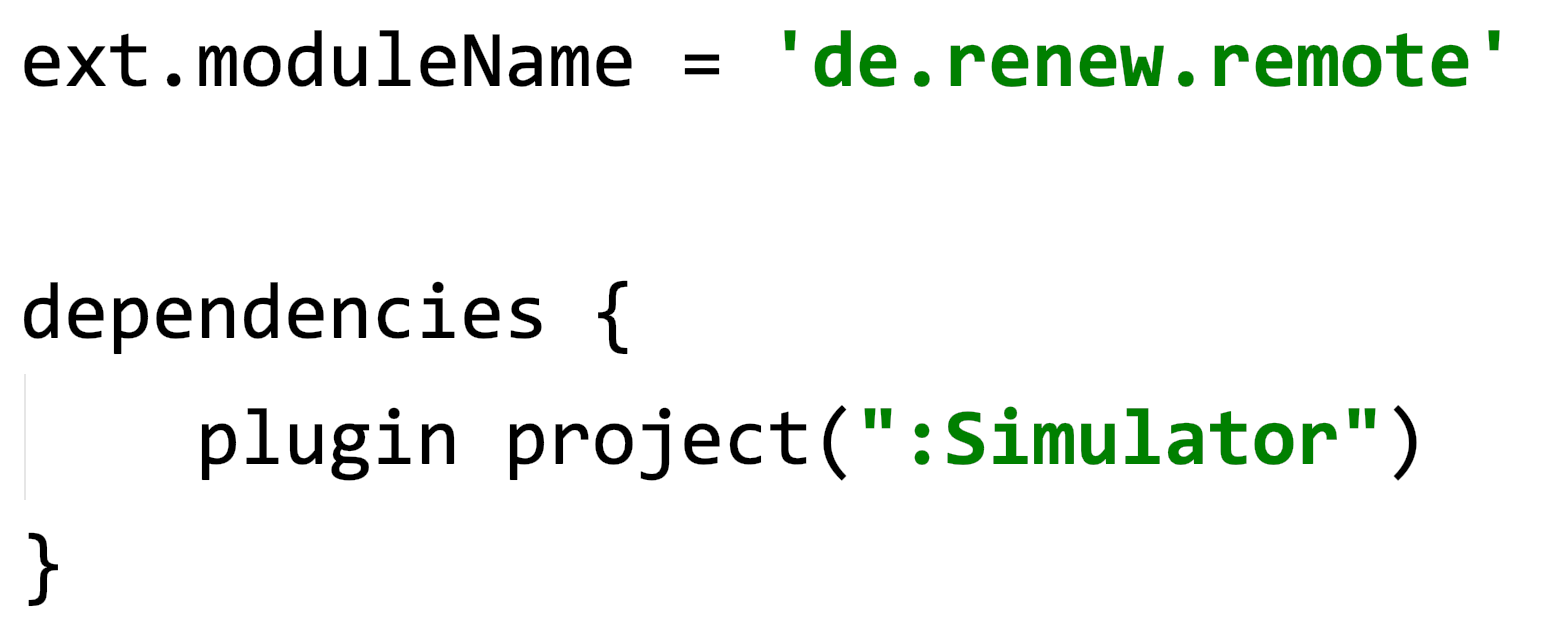
\includegraphics[width=0.5\textwidth]{material/images/Remote_config.png}
	  \caption{Remote Plugin Konfiguration}
	  \label{fig:remote_config}
	\end{figure}	

	Obwohl die globale Konfiguration für die vollständige \textsc{Renew} Version sich steigern wird, deuten die Zahlen auf einen geringeren Code-Abdruck des Gradle \textit{build} Werkzeugs hin.\bigbreak

\subsection{Modulumsetzung} \label{sub:optimierung}% aufwertung
	Nachdem die Modularisierung abgeschlossen wurde, ist eine globale Sicht auf die Umsetzung möglich und offenbart Optimierungspotenzial für die Abstimmung der Modulabhängigkeiten. Zum Beispiel wird das RenewAnt Plugin nur für die Kompilation benötigt und muss nicht für die Ausführung mitgeliefert werden \ref{fig:remote_config}. Daher kann dieses als eine statische Abhängigkeit im Gui Plugin verankert werden und wird der Laufzeit nicht beigefügt.\bigbreak

	\begin{figure}[h!]
	  \centering
	  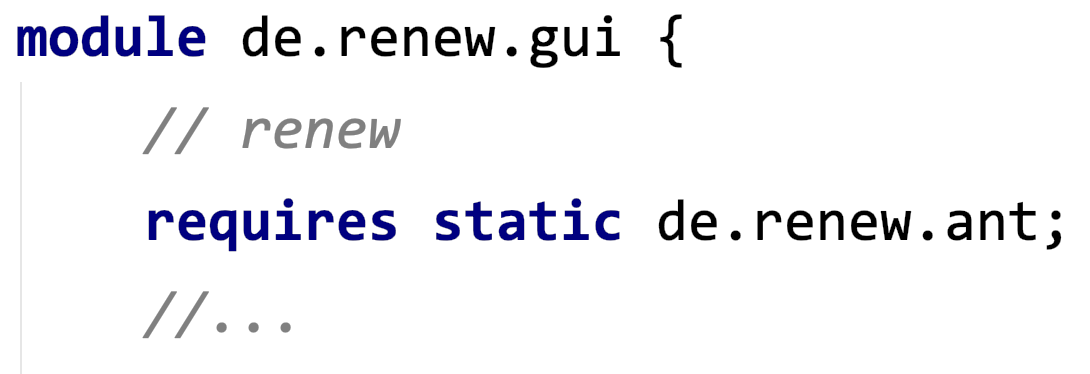
\includegraphics[width=0.4\textwidth]{material/images/gui_config.png}
	  \caption{Statische Konfiguration}
	  \label{fig:gui_config}
	\end{figure}

	Des Weiteren wird klar, dass die \textsc{Renew} Applikation in einer hierarchischen Plugin Architektur aufgebaut ist. Das heißt Plugins, die von anderen Plugins abhängig sind, erfordern das Einbinden aller darunter liegenden Schichten. Dies hat zur Folge, dass das \textit{Util} Plugin in jedem Plugin, das auf diesen und seinen Nachfolger aufbaut, eine Deklaration benötigt. \newline

	Um die Übersicht über die unmittelbar genutzten Module zu behalten, kann mithilfe des \textit{transitiv}  Schlüssels eine angeforderte Bibliothek für alle Nutzer-Plugins offengelegt werden. Demzufolge kann ein Plugin nicht nur ein anderes Plugin erweitern und nutzen, sondern seinen Kontext in die Umsetzung miteinbeziehen. \bigbreak

	\begin{figure}[h!]
	  \centering
	  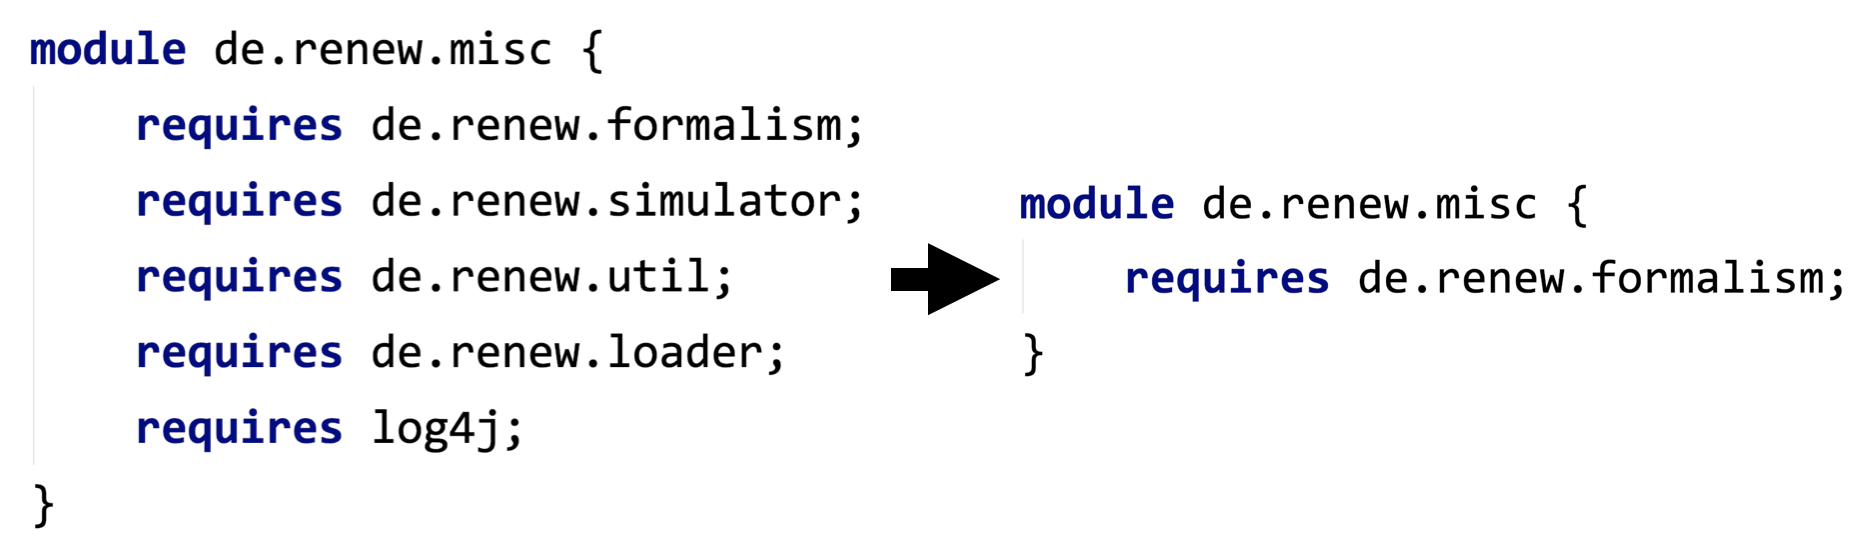
\includegraphics[width=0.8\textwidth]{material/images/misc_trans.png}
	  \caption{Transitive Konfiguration}
	  \label{fig:trans_config}
	\end{figure}

	Um den aktualisierten Java Kontext so gut wie möglich nachzubilden, unterstützt Gradle die Idee der  Modularisierung und dessen Kopplungsarten, indem die Modulkopplung unter Verwendung von unterstützenden API's zum Entwerfen der transitiven und statischen Abhängigkeiten angeboten wird. Diese bestehen aus zwei weiteren Konfigurationspfaden, die durch \textit{api} und \textit{implimentation} gekennzeichnet sind. Die \textit{api} Konfiguration beschreibt eine transitive Abhängigkeit, die durch die Modulhierarchie weitergereicht wird und die \textit{implimentation} Konfiguration, die die genutzten Bibliotheken privat nutzt. Somit können die transitiven \textsc{Renew} Abhängigkeiten, die in der \textit{module-info.java} deklariert sind, auf die Projektstruktur mithilfe von Gradle abgebildet werden.

	\begin{figure}[h!]
	  \centering
	  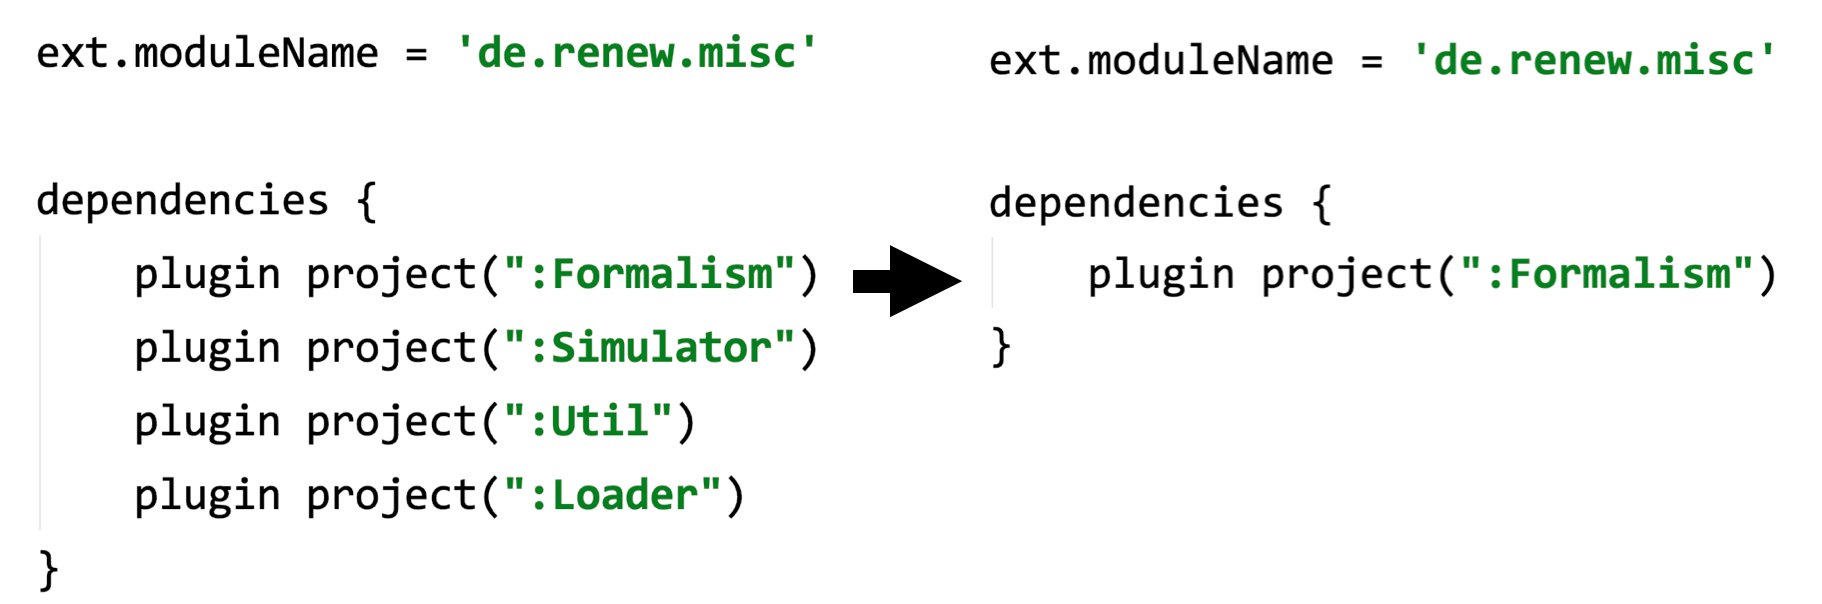
\includegraphics[width=0.8\textwidth]{material/images/gradle_misc.png}
	  \caption{Transitive Gradle Konfiguration}
	  \label{fig:trans_gradle}
	\end{figure}

\subsection{Endergebnis} \label{sub:endergebnis}
	Nachdem \textsc{Renew} verfeinert wurde, entsteht eine eindeutige Darstellung der Plugin Abhängigkeiten und dessen Aufbau. Ersichtlich wird, dass Module eine einfache Art und Wiese bieten, um den Aufbau komplexer Systeme zu verwalten und umstrukturieren.

	\begin{figure}[h!]
	  \centering
	  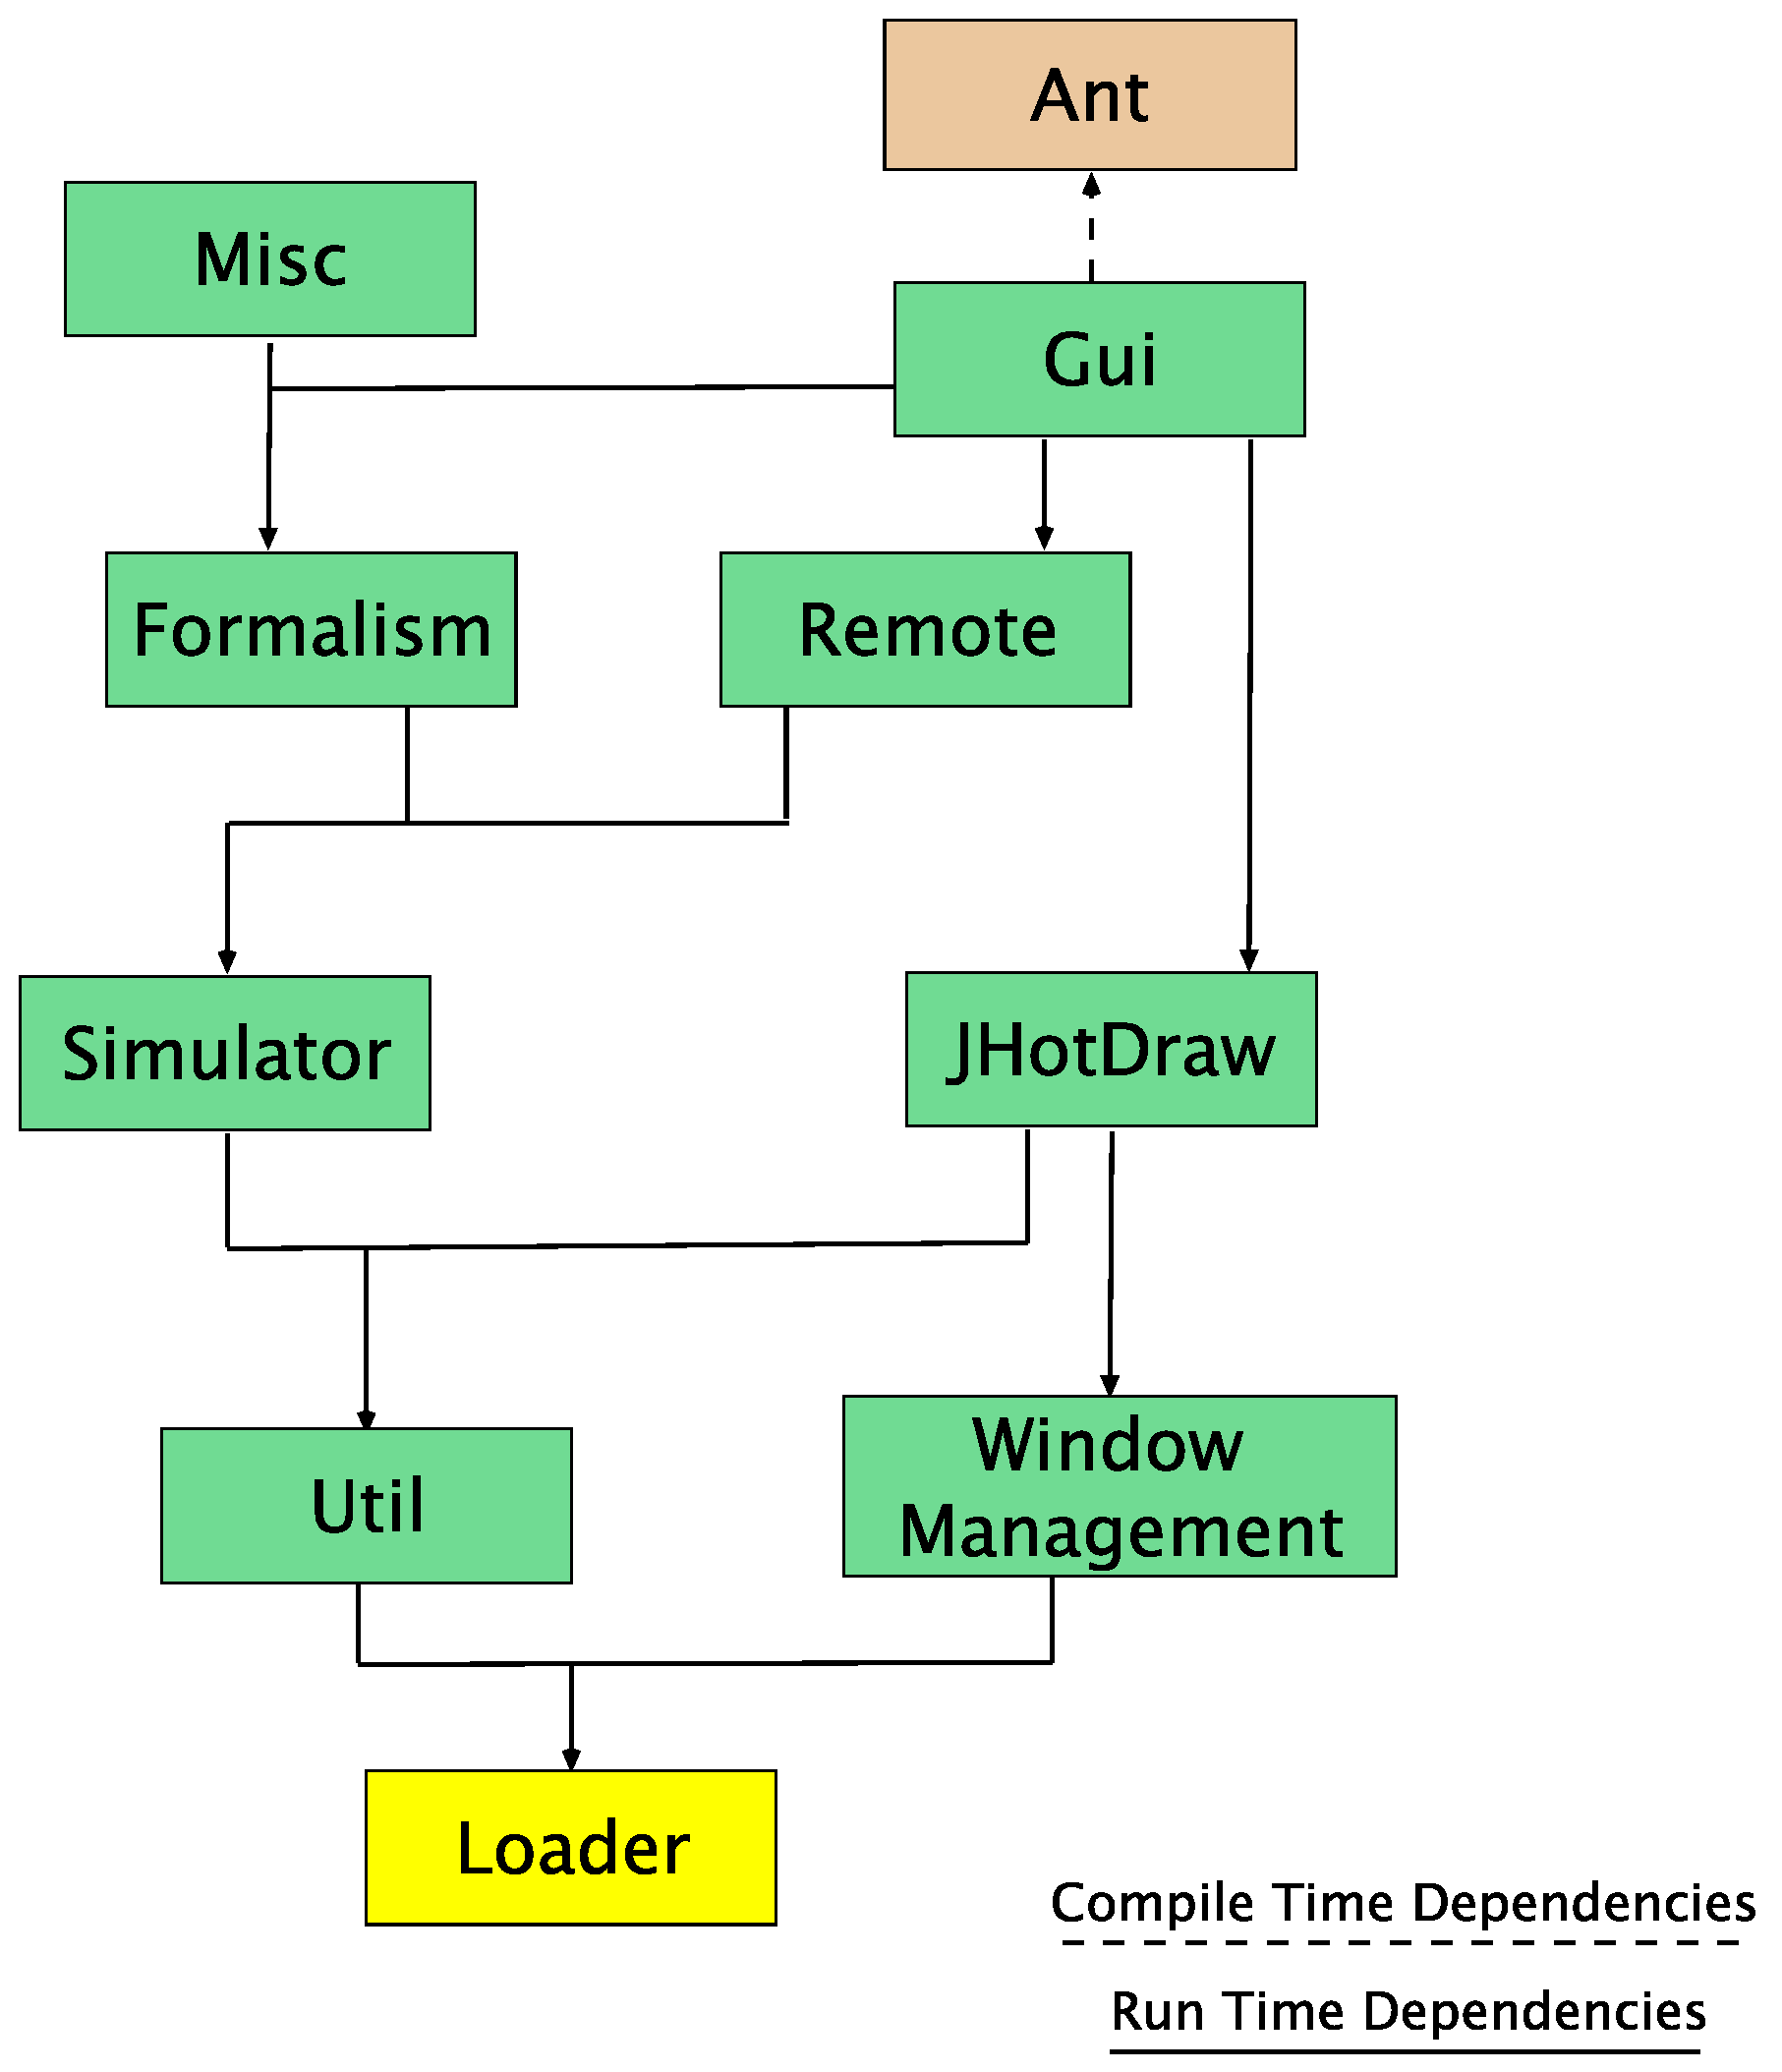
\includegraphics[width=0.8\textwidth]{material/images/renew_plugin_dependencies-migrate_opt.pdf}
	  \caption{Minimale modulare \textsc{Renew} Version}
	  \label{fig:fin_res}
	\end{figure}
% Kritik: Module brauchen explezite schnittstellen, in unseren Fall wurde lediglich die benötigte Logik für die nutzung geöffnet.
% Gradle: Trennen der Klassenpfade hilft die Struktur zu verwalten automatic, plugin, runtime, compile, api und implimentation. 
